
%==============================================================================%
% A PhD thesis template, based on LaTeX memoir class rather than the standard  %
% book class, as memoir offers many additional configuration options.          %
%                                                                              %
% For documentation on the memoir class, and other packages, see:              %
%                                                                              %
%   http://www.ctan.org/search/                                                %
%                                                                              %
% Dave Green --- MRAO --- 2016 September (Version 1.12)                        %
%==============================================================================%
% load the memoir class with basic options ...
%
\documentclass[a4paper,11pt,oneside,extrafontsizes,oldfontcommands]{memoir}
%

% load the thesis package, which sets various options for the memoir
% package, loads other packages (e.g. setting up fonts), and sets up
% various commands ...
%
% note: you will have to edit thesis.sty if you want to change things ...
%
\usepackage{thesis}
%
% other settings...
%
%\listfiles     % uncomment if needed for debugging ...
%------------------------------------------------------------------------------%
% For limited processing, list (with commas) selected files to process...
%
%\includeonly{CHAP-1/chapter1,APP-A/appendixa}
%
\begin{document}
%==============================================================================%
\frontmatter
%------------------------------------------------------------------------------%
\pagestyle{empty}
%
% titlepage ...
%
\ifpdf
  \pdfbookmark[0]{Titlepage}{title}{}
\fi
%
% note: include adjustment of baseline to ensure it looks
%       sensible if it is more than one line long,
%
\begin{center}
 \qquad\\[0mm]
 {\renewcommand\baselinestretch{1.2}\huge\textbf{
%
% if more than one line, use "\\" to start a new line...
%
   Feasibility study on the use of Trigger-Object Level Analysis in the Search for the Standard Model Higgs boson produced by vector-boson fusion and decaying to bottom quarks with the ATLAS detector.
%
 }\par}
 \qquad\\[20mm]
 {\LARGE Andrew J Strange}\\[10mm]
 {\large School of Physics and Astronomy}\\[10mm]
 \includegraphics[width=50mm]{UniOfManchesterLogo.png}\\[30mm]
 {\Large 2018}\\[10mm]
 {\large A dissertation submitted to the University of Manchester \\ for the degree of Master of Science by Research \\ in the Faculty of Engineering and Physical Sciences}
\end{center}

\cleardoublepage

\endinput

%
\pagestyle{plain}
%
% contents ...
%
%
% thesis.sty redefines \baselinestretch for larger line spacings, but
% here do not use this for the table of contents ...
%
\bgroup
\renewcommand{\baselinestretch}{1.0}\normalsize

\tableofcontents

%
% reset to default linespacing ...
%
\vspace{10mm}
WORD COUNT: ???
\egroup

\cleardoublepage

\endinput

%
% declaration ...
%
\chapter*{Declaration}

\addcontentsline{toc}{chapter}{Declaration}

No portion of the work referred to in the dissertation has been submitted in support of an application for another degree or qualification of this or any other university or other institute of learning.

\begin{flushright}
Andrew Strange
\end{flushright}


\cleardoublepage

\endinput

%
% thanks ...
%
\chapter*{Acknowledgements}

\addcontentsline{toc}{chapter}{Acknowledgements}

This dissertation has been produced with guidance and support from many people, without which it would not have seen the light of day.

Primarily, I must thank my supervisor Andy Pilkington. His guiding hand and experience over the course of this project has at times been the only thing keeping it on the straight and narrow. I am indebted to his help and his willingness to put up with me over the course of this year, and this work is built around the backbone he provided.

Secondly, thanks to the Manchester Particle Physics group, for providing a terrific environment for work, for all of the guidance and for all of the socialising. Particular mention must go to my colleagues on the ATLAS project; Jacob, Jonathan
, Yaadav and Agni for all of their invaluable experience and assistance throughout the year. Additionally, I must thank Sabah for providing me with his help and knowledge without hesitation when I needed it.

From my time at undergraduate, I must thank all my friends, who while provided encouragement and support from all the myriad of locations around the world they've run off to, and I must thank my undergraduate Director of Studies, Dave Green, for his advice during my time under his watch and for permitting me to use his \LaTeX template.

Finally however, none of this would have occurred were it not for the support of my dad, mum and brother. Their unwavering and tireless support, endless encouragement and motivating prods and willing to put up with whatever inconvenience I could give them carried this work through to its close.

To all those mentioned here, I owe you the most sincere gratitude. Thank you for everything.
\cleardoublepage

\endinput

%------------------------------------------------------------------------------%
\mainmatter
%------------------------------------------------------------------------------%
% Note: \graphicspaths is set to point to appropriate places to find
% figures for each Chapter or Appendix ...
%
\pagestyle{headings}
%
% chapters ...
%



\graphicspath{{T/FIGS/}{.}}
\chapter{Theory}\label{c:Theory}

\section{Standard Model}


The Standard Model (SM) of particle physics is a collection of several theories which provide the most accurate theoretical framework for describing all known components of matter and their interactions to date. The model describes three fundamental forces, each mediated by an integer spin particle called a \textit{gauge boson}, that control interactions between the spin-$\frac{1}{2}$ \textit{quarks} and \textit{leptons} that make up matter. The mathematical structure is  based on the symmetry group $SU(3)_c\times SU(2)_L\times U(1)_\gamma$ and is required to be gauge-invariant. The SM does not include gravity; gravity cannot be written in the Quantum Field Theories that describe the Standard Model, and gravitational interactions are significantly weaker than the other fundamental forces (Table \ref{t:tab:boson}). As a result, gravitational interactions so are neglected hereafter.

	\subsection{Fermions}

		The full set of spin-$\frac{1}{2}$ \textit{fermions}, described in Tables \ref{t:tab:quark} and \ref{t:tab:lepton}, are the quark and lepton families, which each have three generations. For each distinct particle there is a paired \textit{anti-particle} which is identical aside from opposite charge and \textit{handedness}.

		The handedness or helicity of a particle refers to the projection of the angular momentum of the particle along the direction of the particle momentum. For a spin $\frac{1}{2}$ particle, the angular momentum component can be aligned along the direction of motion (\textit{positive} or \textit{right-handed} alignment) or opposed to it (\textit{negative} or \textit{left-handed} alignment)). This

		Most matter consists of the observable first generation of the up and down quarks and the electron which make up protons and neutrons, along with the unobservable electron neutrino. Both the leptons and the quarks obey Fermi-Dirac statistics. Quarks experience all three fundamental forces, charged leptons interacting via the electromagnetic and weak interactions and neutral leptons experiencing only the weak interaction.

		{
		\setlength{\extrarowheight}{5pt}
		\begin{table}[ht]
			\caption{Spin-$\frac{1}{2}$ fermions: quarks $q$ \cite{pdg}. The top quark mass is taken from direct measurements.}
			\label{t:tab:quark}
			\medskip
			\centering
			\begin{tabular}{clcc}\toprule
				Generation & Flavour & Charge / $e$ & Mass / GeV \\\midrule
				1    &     Up $u$      &    +2/3   & $0.0022\ _{-0.0004}^{+0.0006}$\\
	    &     Down $d$    &    -1/3   & $0.0047\ _{-0.0004}^{+0.0005}$\\
		    	2    &     Charm $c$      &    +2/3   & $1.28\pm0.03$\\
		    	&     Strange $s$    &    -1/3   & $0.096\ _{-0.004}^{+0.008}$\\
				3    &     Top $t$  &   +2/3   & $173.1\pm0.6$\\
	    &     Bottom $b$   &   -1/3   & $4.18\ _{-0.03}^{+0.04}$\\\bottomrule
			\end{tabular}\\[5pt]
		\end{table}
		}
		\begin{table}[ht]
			\caption{Spin-$\frac{1}{2}$ fermions: leptons $l$ \cite{pdg}}
			\label{t:tab:lepton}
			\medskip
			\centering
			\begin{tabular}{clcl}\toprule
				Generation & Flavour & Charge / $e$ & Mass / MeV\\\midrule
				1    &     Electron $e$      &    -1   & $0.5109989461\pm0.0000000031$\\
				&     Electron Neutrino $\nu_e$    &   0  & $<2\times10^{-6}$ \\
				2    &     Muon $\mu$      &    -1   & $105.6583745\pm0.0000024$\\
				&     Muon Neutrino $\nu_\mu$    &    0   & $<2\times10^{-6}$ \\
				3    &     Tau $\tau$  &   -1   & $1776.86\pm0.12$\\
				&     Tau Neutrino $\nu_\tau$   &   0   & $<2\times10^{-6}$ \\\bottomrule
			\end{tabular}\\[5pt]
		\end{table}

		Quarks are always confined into colour singlet \textit{hadrons} bound by the strong interaction, which are either \textit{baryons} ($qqq$) like the \textit{proton} ($uud$) and \textit{neutron} ($ddu$), or \textit{mesons} ($q\bar{q}$) like the positive \textit{pion} ($u\bar{d}$). 

	\subsection{Forces}

		All forces arise due the exchange of unobservable virtual particles, gauge bosons, which obey Bose-Einstein statistics. The three fundamental particle interactive forces for the SM are named the strong, weak and electromagnetic interactions, and are mediated by \textit{gluons}, \textit{weak bosons} and \textit{photons} respectively. The gauge bosons are described in more detail in Table \ref{t:tab:boson}.

		\begin{table}[ht]
			\caption{Spin-1 gauge bosons. The strength of the interaction is typically stated in terms of $\alpha$, a dimensionless constant proportional to the matrix element for the virtual particle exchange for each interaction. For the  The weak interaction is intrinsically stronger than the EM interaction, but the mass of the weak bosons limits the range to extremely short distances.  The strength of gravity is $\sim10^{-39}$ hence it is neglected. \cite{pdg}}
			\label{t:tab:boson}
			\medskip
			\centering
			\begin{tabular}{clclc}\toprule
				Interaction & Particle & Charge / $e$ & Mass / GeV & Strength ($\alpha$) \\\midrule
				Strong    &     Gluon $g$      & 0 & 0 & $\sim1$\\
				Weak (Charged Current)&     $W^+$    &    1   & $80.385\pm0.015$ & \\
				&     $W^-$    &    -1   & $80.385\pm0.015$ & $10^{-6}$ \\
				Weak (Neutral Current)&     $Z$   &    0   & $91.1876\pm0.0021$ & \\
				Electromagnetic (EM)   &     Photon $\gamma$  &  $<1\times10^{-35}$   & $<1\times10^{-27}$ & $\frac{1}{137}$\\\bottomrule
			\end{tabular}\\[5pt]
		\end{table}

		\newpage
		\subsubsection{Quantum Chromodynamics}

		Quantum Chromodynamics (QCD) is the theory of the strong interaction, mediated by the gluon which couples to colour charge. It corresponds to the $SU(3)_c$ symmetry group of the overall SM. The strong interaction conserves energy, momentum, angular momentum and colour charge. Only quarks and gluons themselves possess colour charge, so while quarks are the only fermion to feel the strong interaction, gluons can self-couple.

		\subsubsection{Electroweak Unification}

		Electroweak Unification (EW) is the expression of the electromagnetic interaction and the weak interaction as separate manifestations of a combined electroweak force in the Glashow-Weinberg-Salam model \cite{gws-g, gws-w, gws-s}, which corresponds to the $SU(2)_L\times U(1)_\gamma$ symmetry group. Quantum Electrodynamics (QED) describes the macroscopically observable $U(1)$ electromagnetic force  with the photon as the mediating boson, and any interaction conserves energy, momentum, parity and charge and additionally never changes particle type through the interaction. The $SU(2)$ weak interaction is mediated by the charged current vector bosons $W^+$, $W^-$ and the neutral current vector boson $Z$, which have large masses that limit the weak interaction to very short distances. The charged current interaction is capable of changing the flavour of a particle and also of violating parity in an interaction.

		The weak interaction by itself was observed to diverge from observation at high energies, leading to the introduction of the unified theory. The combined  $SU(2)_L\times U(1)_\gamma$ group produces four gauge bosons which mix to produce the more recognisable $\gamma$, $W^+$, $W^-$  and $Z$ bosons. The unified force couples to weak isospin, which allows self-coupling between the massive vector bosons, but not the photon as it does not carry electric charge.

		While the weak interaction acts on both quarks and leptons, the quark sector is affected by the distinction between the mass and flavour eigenstates of quarks. The physically observed flavour eigenstates are distinct from the quark eigenstates of the weak interactions, which are superpositions of the mass eigenstates. The effect of this quark mixing in the weak interaction is that different flavour changing interactions have different strengths. The mixing of the mass eigenstates ($q$) into weak eigenstates ($q^\prime$) is described by the Cabbibo-Kobayashi-Makasawa matrix \cite{ckm-c, ckm-km}:

		\begin{equation}
		\begin{pmatrix}
		d^\prime \\
		s^\prime\\
		b^\prime \\
		\end{pmatrix}
		 = \begin{pmatrix}
		V_{ud} & V_{us} & V_{ub} \\
		V_{cd} & V_{cs} & V_{cb} \\
		V_{td} & V_{ts} & V_{tb} \\
		\end{pmatrix}
	    \begin{pmatrix}
	    d \\
	    s\\
	    b \\
	    \end{pmatrix}
		\end{equation}



	\subsection{Spontaneous Symmetry Breaking: The Higgs Boson}
	\label{t:symbreak}


	In addition to the forces, particles acquire mass by coupling to the \textit{Higgs} field via the spin-$0$ Higgs boson \cite{gauge-boson-mass, higgs-1, higgs-2}, which is covered in more detail in Section \ref{t:symbreak}.

	OUT OF PLACE

	The gauge field theories used for the QCD and EW models when unaltered require massless gauge bosons in order to preserve gauge invariance, which follows from the Klein-Gordon equation:
	\begin{equation}
		\frac{\partial^2\psi}{\partial t^2} = (\nabla^2 - m^2)\psi
	\end{equation}
	 This is satisfactory for the gluon and photon, but a separate theory is required to explain the mass of the $W^\pm$ and $Z$ bosons. The Higgs Mechanism proposed introducing a scalar field that interacts with the $W^\pm$ and $Z$ fields. In the Lagrangian formulation this results in a term akin to a mass term ($\propto\psi^2$) which effectively links that mass of the bosons to their coupling with this scalar field. This addition to the Lagrangian is still required to preserve the symmetry of the system and respect the gauge invariance, but is also required to have a non-zero expectation value for the field in the vacuum or ground state of space. The Higgs mechanism introduces the scalar field $\phi$ which has a potential energy $V(\phi)$:
	 \begin{equation}
		 V(\phi) = a\phi^4 - b\phi^2
	 \end{equation}

	This results in an equilibrium point ($\phi=0$) that respects the symmetry, but is inherently unstable, with an infinite set of degenerate non-zero minima at $|\phi^2|=\frac{b}{2a}$ where the symmetry is \textit{spontaneously} broken. This field, in an analogous fashion to the other quantum fields of the SM, can produce particles from excitations which form the physical \textit{Higgs Scalar Boson} $H$. Confirmation of the Higgs boson as part of the SM was only achieved relatively recently \cite{higgs-atlas, higgs-cms}, where a spin-$0$ boson consistent with the SM Higgs was observed. Subsequent measurements made have provided agreement on the new particle as the Higgs boson with a mass of $125.09$\,GeV \cite{pdg}. Section \ref{t:higgs} covers in more detail the production and behaviour of the Higgs boson in collider experiments.


\section{Physics of \textit{pp} Collisions}

	Recent experimental efforts to probe the Standard Model have focused on high-energy collider experiments, where beams of particle with equal energy are collided head on within detectors.  For proton-proton ($pp$) collisions, matters are complicated as the colliding protons are composite particles, which at high energy consist of the three \textit{valence} quarks and a sea of virtual quarks and gluons. Collectively these constituents are referred to as \textit{partons} where each parton carries a fraction of the overall hadron momentum, and the interaction in the $pp$ collision consists of elastic scattering between these partons. At a given energy scale $Q^2$ the probability that a parton $i$ carries a fraction $x_i$ of the overall momentum is described by the parton distribution function (PDF) $f_i(x, Q^2$). These PDFs cannot be calculated from QCD but can be determined from experimental measurements, and collections of PDFs have been assembled from the leading collider experiments \cite{pdfs}.

	In any particle interaction, the probability a particular reaction occurs is in proportion to the cross section of the reaction. The cross section for a short range, hard parton-parton collision is given by $\hat{\sigma}(Q^2)$, where scattering energy scale $Q^2 = x_1x_2E^2_{cm}$ in the parton-parton centre-of-mass frame where $E_{cm}$ is the energy in the centre-of-mass frame. To compute the cross section $\sigma$ for some hard process $pp\rightarrow X$, all possible combinations of incoming partons must be summed over and the momentum fractions integrated over while accounting for the PDFs:
	\begin{equation}
	\sigma = \sum_{i, j = q, g} \int dx_1dx_2f_i(x_1, Q^2)f_j(x_2, Q^2)\hat{\sigma}(Q^2)
	\end{equation}

	\subsection{Geometry}
	\label{t:geometry}

	The high energy protons used in collisions are relativistic in nature, and as the momenta of the colliding partons are not guaranteed to be equal and opposing there is always an unknown element of longitudinal boosting in $pp$ collisions. As a consequence, use of light-cone coordinates and some definitions of convenient quanties can be of benefit to $pp$ collision analyses \cite{lightcone-all-that}.

	Typically the momentum in the transverse plane \pt is used for a particle, and the rapidity $y$ of a particle with non-zero \pt is defined:
	\begin{equation}
	y = \frac{1}{2}\ln\frac{E+p_z}{E- p_z}
	\end{equation}

	This rapidity $y$ transforms additively to boosts along the $z$ axis, so any rapidity difference between two objects is invariant to such boosts. For cases where the mass of a particle is negligible (highly relativistic particles) the rapidity can be related to the polar angle of the particle as the pseudo-rapidity $\eta$:
	\begin{equation}
	\eta = -\ln\tan\frac{\theta}{2}
	\end{equation}

	The distance between two objects within the detector is commonly expressed in the ($\eta$, $\phi$) space rather than absolute, with this separation being given by $\Delta R = \sqrt((\Delta\eta)^2 + (\Delta\phi)^2)$

	\subsection{Collision simulation}

	A $pp$ collision is a complex event which results if a significant number ($\mathcal{O}(1000)$) of final state particles, each of which interact and evolve over the timescale of an event. This progression of the collision event can be broken down into distinct stages of behaviour of the produced particles: the \textit{hard process}, \textit{parton shower}, \textit{hadronisation}, \textit{unstable particle decays} and \textit{underlying event}.

	This breakdown is key to the simulation of $pp$ collisions using Monte-Carlo event generators, the use of which is critical in current high energy physics research. Monte-Carlo simulations of collisions are used to predict and prepare for real data-taking experiments, obtain control datasets of particular particle interactions and act as controls to optimise analysis tools. The breakdown of the interaction into distinct stages has allowed specialised software to be produced for each step, which makes use of a characteristic scale and certain safe approximations for the step to provide reliable predictions, while reducing the computational demands of the simulation \cite{monte-carlo}.

		\subsubsection{Hard Process}

			The first stage of a $pp$ collision and the first step of a simulation, the hard scatter refers to highest momentum transfer process in the event between coloured particles, and forms the core of the event. This details the interaction of partons entering the event and those outgoing partons resulting from the process. In simulation the probability distribution of the partons is calculated from perturbation theory to the desired accuracy (LO, NLO etc) using the PDFs of the constituents.

		\subsubsection{Parton Shower}

			While the hard scatter interaction in a collision is relatively straightforward, the overall behaviour of the partons is much more complex as they progress through the event. The incoming and outgoing partons from the hard scatter radiate additional interaction particles during the event
			The Bremsstrahlung  radiation of photons by scattered electric charges is well described by QED, and the analogous radiation of gluons by scattered colour charges as explained by QCD produces additional partons within the interaction. However, as the gluons produced by QCD scattering themselves carry colour charge, there is extending showering of gluons producing gluons, resulting in the phase space of the interaction being filled with a sea of soft gluons. Both of these radiative processes make up the parton shower stage of the event simulation.

			The evolution of these parton showers is evaluated in Monte-Carlo simulations using a step-by-step iterative process, on the scale of momentum transfer in the interaction. This process is started at the hard scatter and evolved through the interaction with decreasing momentum scale until the point at which perturbation theory breaks down, necessitating a different evaluation method.

		\subsubsection{Hadronisation}
		\label{t:hadronisation}

			With the breakdown of perturbation theory at low momentum scales,  observable colourless hadrons are constructed from the coloured partons using hadronisation models in order to extend the simulation. These hadrons are the physical final state particles observed in the detector, which exist due to the colour confinement of the quarks and gluons. Within a particle detector, rather than individual hadrons \textit{jets} of hadrons are observed. As a coloured fragment produced in the interaction moves away from the interaction, it will create other coloured fragments around itself in order to produce a confined hadron while moving away from the collision. This occurs repeatedly for each hadron ejected from the collision as it moves away, producing a collimated stream of hadrons which make up a jet.

			In simulation this step involves collecting the partons produced in the parton shower into hadrons, and is typically evaluated using either a String model \cite{stringmodel} or a Cluster model \cite{clustermodel}. These steps are models, and not calculations as to how the partons combine, as to calculations being prohibited by the breakdown of perturbation theory.

		\subsubsection{Unstable Particle Decays}

			The final stage of the evolution of the parton shower considers the hadrons produced during the shower. These hadrons may not be stable particles but could be resonances that go on to decay within the detector to produce the more stable hadrons observed in the data. Most modern simulation software models these decays, but the exact specification of the decay tables and channels has a significant impact on the final state of the simulation.

		\subsubsection{Underlying Event}
		\label{t:underlying}

			While the hard scatter and subsequent parton shower results from the highest momentum interaction of the $pp$ collision, the remnants of the proton not involved in this will continue to interact with each other. This produces additional soft hadrons that fill the interaction environment, overlapping with the products of the hard scatter interaction.

			The dominant model for simulation of the underlying event is a perturbative model where the other components undergo additional discrete hard scatter interactions and corresponding parton showers which are simulated in an corresponding fashion to the core scattering.

	\subsection{Monte-Carlo Software}

		There is a broad selection of software tools for evaluating $pp$ collisions, from general purpose simulations like \textsc{Pythia}\cite{pythia} or \textsc{Sherpa}\cite{sherpa} which are used to evaluate the complete process, to more specific tools like \textsc{Powheg}\cite{powheg} which is used to produce hard scatter events with NLO matrix elements. Most software packages make use of the chain of generation for an event outlined previously, and modern analyses will make use of multiple generators interfaced together to compute different steps with improved accuracy.

\section{The Higgs Boson}
\label{t:higgs}

	Detecting the SM Higgs boson is strongly dependent on the predominant production and decay channels for the Higgs boson, which in turn depend on the specifications of the collider used for the search. In this section the relevant production and decay channels at the Large Hadron Collider (LHC) will be discussed.

			\begin{figure}[h]
				\centering
				\includegraphics[width=0.7\linewidth]{T/FIGS/YRHXS_Summary_fig3}
				\caption{SM Higgs Production cross section for $\sqrt{s}=14$ TeV. $\,pp\rightarrow H$ corresponds to gluon-gluon fusion production and $pp\rightarrow qqH$ vector boson fusion. \cite{LHCHiggsCS}}
				\label{fig:higgsproductionCS}
			\end{figure}

	\subsection{Higgs Production}

		While there are many various methods for production of a Higgs boson, at the LHC the cross section is dominated by gluon-gluon fusion (\ggF) as shown in Figure \ref{fig:higgsproductionCS}, with the second largest cross-section arising from Vector Boson Fusion (VBF, Section \ref{t:VBF}). Other significant production processes are the associated production with a weak boson ($WH/ZH$, Higgs-strahlung) production modes and associated production with top quarks ($ttH$) \cite{LHCHiggsCS}. The lowest order Feynmann diagrams for these processes are shown in Figure \ref{fig:higgsproddiag}.

			\begin{figure}[h]
				\centering
				\includegraphics[width=0.5\linewidth]{T/FIGS/ggf}
			\end{figure}
			\begin{figure}[h]
				\centering
					\begin{minipage}[h]{0.4\linewidth}
						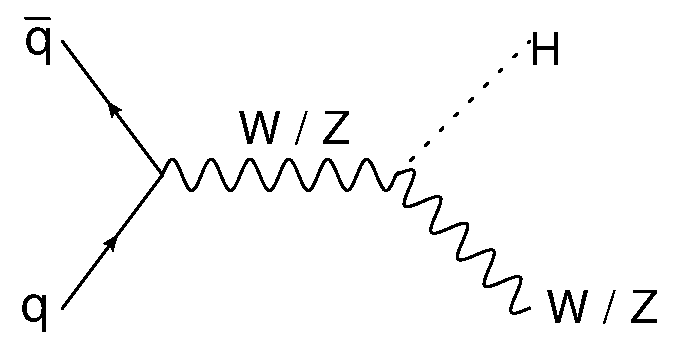
\includegraphics[width=1\linewidth]{T/FIGS/whzh}
					\end{minipage}
					\quad\quad
					\begin{minipage}[h]{0.4\linewidth}
						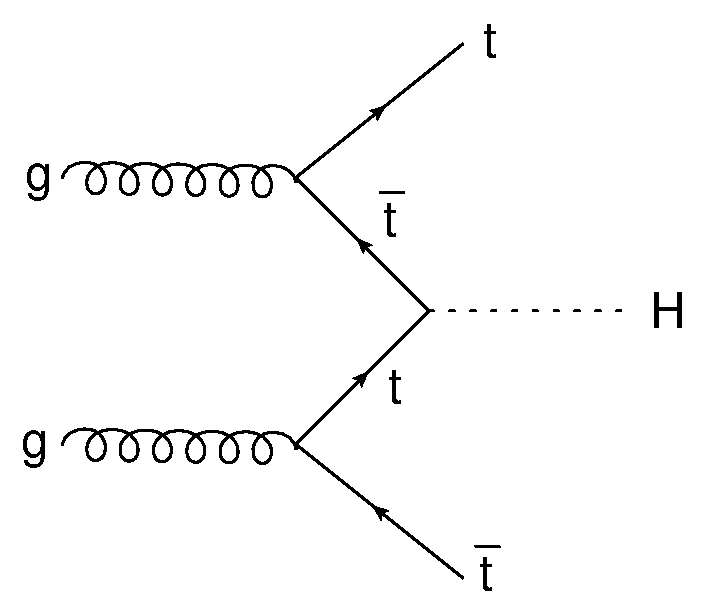
\includegraphics[width=1\linewidth]{T/FIGS/tth}
					\end{minipage}
				\caption{Lowest order Feynmann diagrams for gluon-gluon fusion (\ggF), $W/Z$ associated production ($WH/ZH$) and top anti-top associated production ($t\bar{t}H$).}
				\label{fig:higgsproddiag}
			\end{figure}


		\subsubsection{Gluon-gluon Fusion}

		The dominant production mechanism for the Higgs boson in hadron colliders is the \ggF\, production via in intermediate quark loop. The dynamics of this mechanism are controlled by strong interactions, thus calculations of QCD corrections are necessary for any accurate predictions, and have been computed up from next-to-leading order (NLO) to N$^3$LO for the \ggF process in recent years, along with the inclusion of Electro-Weak corrections in the cross section calculations \cite{LHCHiggsCS}.

	\subsection{Vector Boson Fusion}
	\label{t:VBF}

		Production of a Higgs boson from the fusion of vector bosons radiated from initial-state quarks is the second largest cross-section at the LHC, and is useful as a production mode due to topological characteristics which can distinguish the event from \ggF. In \VBFHBB, the characteristic topology is a pair of
		central \bjets forming the Higgs candidate, and two forward, close to the beam line VBF jets formed from remnants of the initially colliding protons as displayed in Figure \ref{fig:T:vbf}. In addition central jet activity is suppressed due to the lack of colour exchange between the colour single Higgs boson and the decay \bquarks \cite{VBF2004}.  These distinct features mean that while the cross section for VBF at a Higgs mass of $< 200$ GeV is dominated by \ggF, the easy to detect signature means the channel is a cornerstone of searches for the Higgs boson.

		\begin{figure}[h]
			\centering
			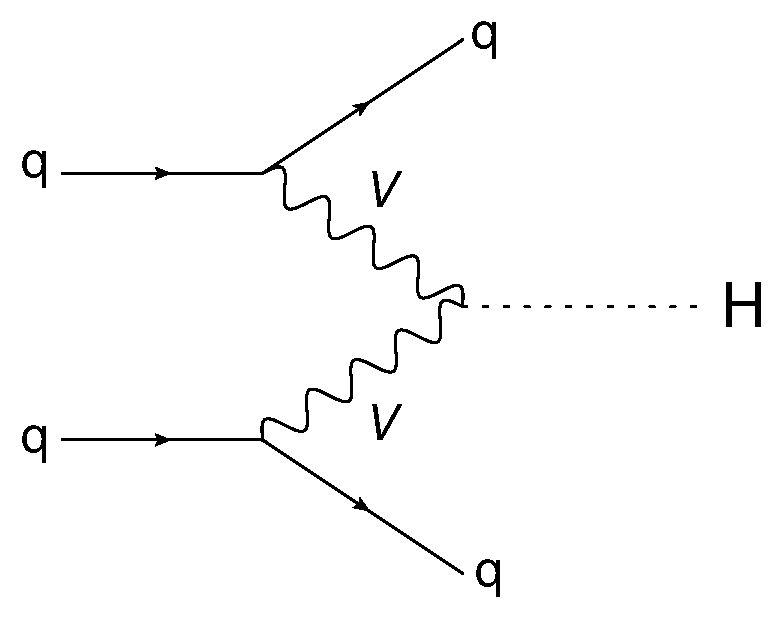
\includegraphics[width=0.4\linewidth]{T/FIGS/vbf}
			\caption{Feynmann diagram for the production of a Higgs boson via Vector Boson Fusion, where $q$ denotes any quark or antiquark}
			\label{fig:T:vbf}
		\end{figure}


	\subsection{Higgs Decay}

		The branching ratios for decays of the Higgs boson in the Standard Model have been extensively determined using Monte-Carlo event generators. As is to be expected, the relative cross-sections of the decay modes are strongly dependent on the mass of the Higgs boson, as highlighted in Figure \ref{fig:higgsbrlm}.

		\begin{figure}[h]
			\centering
			\includegraphics[width=0.5\linewidth]{T/FIGS/Higgs_BR_LM}
			\caption{Higgs decay branching ratios for the low mass region with their uncertainties \cite{LHCHiggsXS2013}.}
			\label{fig:higgsbrlm}
		\end{figure}

		\newpage
		While observations consistent with the Standard Model Higgs boson have been made for the $H\rightarrow \gamma\gamma$, $H\rightarrow ZZ$, $H\rightarrow W^+W^-$ and $H\rightarrow \tau^+\tau^-$ channels, observation of th $H\rightarrow bb$ decay channel is significantly hindered owing to the large background from multijet production in hadron collisions. Despite this, the topology of the VBF production mechanism makes it a viable option for observation of the  $b\bar{b}$ decay channel.

	\subsection{VBF Searches}

		Searches fo the \VBFHBB\, interaction look for a resonance in the invariant mass of a pair of jets containing \bquarks ($m_{bb}$) in events with the characteristic topology. This characteristic topology distinguishes the signal events from the multijet events that form the dominant background with a non-resonant $m_{bb}$ spectrum. An additional resonant background contribution to the \mbb spectrum is due to decay of a $Z$ boson to two jets in association with two jets.

		In the most recent searches for the Higgs boson produced via VBF, which this analysis emulates, the \VBFHBB\, events are indistinguishable from the \ggF\, events, and are separated using a multivariate boosted decision tree (BDT) analysis to refine the phase space to the most VBF sensitive BDT regions.


\endinput


\graphicspath{{D/FIGS/}{.}}
\chapter{Detector}\label{c:Det}

\section{The Large Hadron Collider}

\section{The ATLAS Detector}

\section{Triggers}

\section{Object Reconstruction}
	
	\subsection{Jets}
	
	\subsection{\bjets}

\section{\textit{b}-Tagging}
\label{det:btagging}

	Identification of \bquark jets in ATLAS is based on combining the output of three separate \btag algorithms: Impact Parameter based (IP2D and IP3D, described in Section \ref{det:btag:ip}), Secondary Vertex based (SV, described in Section \ref{det:btag:sv}) and Decay Chain based (JetFitter, described in Section \ref{det:btag:jf})into a multivariate discriminant (MV2, covered in Section \ref{det:btag:mv}) which is used to distinguish the jet flavours. These algorithms have undergone continuous improvement over the Run-2 cycle of the LHC to improve the separation of jet flavours. 
	
	\subsubsection{IP2D and IP3D: Impact Parameter based Algorithms}
		\label{det:btag:ip}
		
		The typical topology for a \bhadron of a secondary vertex displaced from the hard scatter interaction point as a results of the lifetime of \bquark is used as the basis of these algorithms. Impact parameters of tracks from the secondary vertex are computed with respect to the primary vertex of the interaction. The IP2D algorithm uses a transverse impact parameter ($d_0$) defined as the distance of closest approach of a track to the  primary vertex in $r$-$\phi$ plane around the vertex. The IP3D algorithm uses both the transverse and a correlated longitudinal impact parameter ($z_0\sin\theta$), defined as the distance between the point of closest approach in $r$-$\phi$ and the primary vertex in the longitudinal plane. \todo{I kind of want a diagram here, but that doesn't appear to be the norm}. These parameters typically have large values as a result of the lifetime of \bquark. The signs of the impact parameters are also defined to take account of if they lie infront or behind the primary vertex with respect to the jet direction, with secondary vertices occuring behind the primary vertex normally due to background.
		
		The significance of the impact parameter values ($\frac{d_0}{\sigma_{d_0}}$, $\frac{z_0}{\sigma_{z_0\sin\theta}}$) for each track are compared to probability density functions obtained from reference histograms derived from Monte Carlo simulation, with each track being compared to a selection of reference track categories. This results in weights which are combined using a log-likelihood ratio (LLR) discriminant to compute an overall jet weight separating the $b$, $c$, and light-jet flavours from each other. \cite{btagOptimisation, bTagPerformance}
		
	\subsubsection{SV1: Secondary Vertex Finding algorithm}
	\label{det:btag:sv}
	
		The secondary vertex algorithm uses the decay products of the \bhadron to reconstruct a distinct secondary vertex. The algorithm uses all tracks that are significantly displaced from the primary vertex associated with the jet, forming vertex candidates for all pairs of track, while rejecting any vertices that would be associated with decay of long lived particles (e.g. $K_s$, $\Lambda$), photon conversions or interactions with the material in the detector. The tracks forming these vertex candidates are then iteratively combined and refined to remove outliers beyond a $\chi^2$ threshold leaving a single inclusive vertex.
		
		The properties of this secondary vertex are used to differentiate the flavour of the jet. The SV1 algorithm is based on a LLR formalism similar to the IP algorithms, and makes use ot the invariant mass of all charged tracks used to reconstruct the vertex, the number of two track vertices and the ratio of the invariant mass of the charged tracks to the invariant mass off all tracks. In addition the algorithm is signed in a similar fashion to the IP algorithms and uses the $\Delta R$ between the jet direction and secondary vertex displacement direction in the LLR calculation. The algorithm uses distributions of these variables to distinguish be      tween the jet flavours. \cite{btagOptimisation, bTagPerformance} \note{Might be worth mentioning the way these are trained}
		
	\subsubsection{JetFitter: Decay Chain Multi based Algorithm}
	\label{det:btag:jf}
	
		The JetFitter algorithm exploits the topological structure of weak \bhadron and \chadron decays inside the jet to reconstruct a full \bhadron decay chain. A Kalman filter \todo{Either understand or just cite} is used to find a common line between the on which lie the $b$, $c$ and primary vertices to approximate the \bhadron flight path. A selection of variables relating to the primary vertex and the properties of the tracks associated with the jet are used as input nodes in a neural network. This neural network uses the input variables and \pt and $|\eta|$ variables from the jets, reweighted in the kinematic variables to ensure the spectra of the kinematics are not used in the training of the neural net. The neural network outputs a discriminating variable relating to each jet flavour which are used to tag the jets. \cite{btagIdentification}
		
	\subsection{Multivariate Algorithm}
	\label{det:btag:mv}
	
	The output variables of the three basic algorithms described prior are combined as input into the Multivariate Algorithm MV2. MV2 is a Boosted Decision Tree (BDT) algorithm which has been trained on $t\bar{t}$\note{Why?} events to discriminate \bjets from light and \cjets. The algorithm makes use of the jet kinematics in addition to the tagger input variables to prevent the kinematic spectra of the training sample from being used as discriminating factor. \note{list all input variables?} The MV2 algorithm is an revised version of the MV1 algorithm used during Run-1 of the LHC, and has three sub-variants (MV2c00, MV2c10, and MV2c20) of the algorithm distinguished by the exact background composition of the training sample. The naming convention initially referred to the \cjet composition of the training sample, e.g. for MV2c20 the \bjets are designated as signal jets where a mixture of 80\% light jets and 2-\% \cjets was designated as background. 
	
	The MV2 algorithm has a set of working points, defined by a single value of the output distribution of the algorithm, which are configured to provide a specific \bjet selection efficiency on the training $t\bar{t}$ sample. Rather than being used independently, physics analyses will make use of several working points as an increase in \bjet efficiency (corresponding to \textit{looser} \bjet selection) will bring an increased mistag rate of light and \cjets.
	
	These algorithms were refined prior to the 2016 Run-2 data-taking session in response to \cjets limiting physics analyses more the light-jets. This change  to enhance the \cjet rejection meant that for the MV2c10, the \cjet fraction was set to 7\% in training and the fraction for MV2c20 was 15\%. There were a selection of other improvements to the algorithm made to the algorithm relating to the BDT training parameters and the use of the basic algorithms before the 2016 data taking. With these refinements, the MV2c10 algorithm was found to provide a comparable level of light-jet rejection to the original 2015 Mv2c20 algorithm with impoved \cjet rejection, so was chosen as the standard \btagging algorithm for 2016 analyses. \cite{btagOptimisation}
	
	
	
	
	
\endinput


\graphicspath{{ES/FIGS/}{.}}
\chapter{Event Selection}\label{c:ES}

	This chapter is dedicated to describing the selection criteria for real and simulated event data used in the analysis, along with the specific calibrations and configurations used in the extraction and reconstruction of the objects making up the analysis. The event selections described here were chosen to target the analysis towards the typical \VBFHBB\, final state described in Section \ref{t:VBF}.

	\section{ATLAS Event Data}

	The raw data from the ATLAS detector is stored in a proprietary data format used by the ATLAS experiment, the Analysis Object Data (AOD) format. This is the output of the event reconstruction software on an event by event basis. For Run-2 of the LHC experiment, this was upgraded to the xAOD format, which is readable by ROOT \cite{ROOT}, a modular software framework managed by CERN and designed specifically for analysis of large datasets with complex statistical analysis, visualisation of data and storage. The xAOD format is a many leveled branching tree structure, with nodes of the tree grouping together related information from each event, and has an associated Event Data Model (EDM) to standardise classes, interfaces and types for representation of an event to facilitate simple analysis \cite{xAOD}.

	Analyses typical make use of a derivation framework to refine the complete xAOD into a more selective Derived xAOD (DxAOD) which will normally contain only the relevant objects to a target analysis, and results in a smaller dataset that is much easier to manipulate, store and operate over. These derivations are produced using the ATLAS bulk data processing framework Athena \cite{athena}, and analysis make use of the internal AnalysisBase suite of tools to perform research studies. This analysis was conducting using the EventLoop package for event processing.

	This framework is used for both the real event data and the simulated Monte-Carlo data, with DxAODs of both datasets being used as the core data for any ATLAS physics analysis. These datasets, following from the large output rate of the LHC, are extremely large, necessitating the use of parallelised computation to perform any statistically significant analysis. The computational framework developed at ATLAS is designed to perform concurrent computation, and processing makes use of the Worldwide LHC Computing Grid \cite{grid} to perform the analysis.


	\section{Event weights}

		 In order to accurately compare the simulated events from the Monte-Carlo samples with the real event dataset, it is necessary to normalise the Monte-Carlo samples to the total luminosity of the dataset, based on the theoretical cross-section for the interaction. The Monte-Carlo simulation assigns a weight $w_i$ to each event simulated, which are summed to give the total number of events in the Monte-Carlo. Each bin in results produced from the simulated data is reweighted using a scaling factor:

		 \begin{equation}
		 w_{MC} = \frac{\sigma k L}{N}
		 \end{equation}

		 where $\sigma$ is the theoretical cross section, $L$ the integrated luminosity of the real dataset, $N$ the total number of simulated events ($\Sigma_N w_i$) and $k$ the Real $K$-Factor, which is a correction to the leading order cross section to reproduce the higher order calculation for the interaction.


	\section{Samples}
		 Real event data was taken from the 2016 13 TeV run, with Data Period D used owing to limited storage space on analysis computing facilities. The \texttt{HIGG5D3} derivation was used for the data and Monte-Carlo sample, a full list of tags and files is given in Appendix \ref{a:config}. This analysis used the all year 25ns Good Runs List (Table \ref{t:files}), resulting a a data luminosity of $4.6312$b$^{-1}$. The simulated VBF sample (Table \ref{t:files}) was produced during the MC15c production period. The sample was produced using the NLO generator \textsc{powheg} configured using the CTEQ6L1 \cite{CTEQ} set of PDFs and interfaced with \textsc{pythia8} tuned to AZNLO \cite{AZNLO}.

	\section{\VBFHBB\, Analysis Strategy}
		 Following from the description of the \VBFHBB\, events in Section \ref{t:VBF}, target events are selected by requiring two central \bjets which form the Higgs candidate and two high \pt VBF jets. Searches using \VBFHBB consider two exclusive analysis channels of interesting events:, the \textit{four-central} channel requires all four jets to be contained within the central region $|\eta| < 2.8$ and the \textit{two-central} channel requires two jets in the central region and one forward jet. In this study, the online trigger level jets could not be extracted for the specific trigger chains used previously for the \textit{four-central} channel, so analysis focuses on the \textit{two-central} channel.

		For the \textit{two-central} channel, the event was required to pass the \texttt{HLT\_j80\_bmv2c2070\_split\_\-j60\_bmv2c2085\_split\_j45\_320eta490} trigger. This trigger requires a single L1 jet ROI of $E_\text{T} > 40$GeV and $|\eta| < 2.5$. In addition, a second central jet ROI with $E_\text{T} > 25$ and a forward jet ROI with $E_\text{T} > 20$GeV and $3.1 < |\eta| < 4.9$ are both required.
		At the HLT level, one central jet \btagged\, at the \textit{tight} working point with \pt $>80$GeV, and a jet with \pt$>60$GeV tagged at the \textit{loose} working point. finally a HLT forward jet with $E_\text{t}>45$ between $3.2 < |\eta| < 4.9$.

		Once the trigger was passed, the event was required to contain one jet with \pt$>95$GeV which was \btagged at the \textit{tight} working point and one additional jet with \pt$>70$GeV that passed the \textit{loose} \btag working point. One forward jet with $3.2 < |\eta| < 4.4$ and \pt$>60$GeV was required along with a final VBF jet with \pt$>20$GeV and $|\eta| < 4.4$. Finally the \pt of the $bb$ pair was required to exceed 160 GeV. (This is to remove sculpting EXPLAINNNN)


NOTES:
what do we need in this sectionL:
	xAODs
	offline recovery
	online recover
	central channels
	triggers used






	\section{Jet Extraction}

		The analysis is based on the jet objects reconstructed from the detector contained in the DxAOD. Both the offline jet objects and the online equivalents are retrieved, however the method by which the full collection of jets is assembled differs between each case. For offline jet objects, the DxAOD contains a complete set of jets for each reconstruction algorithm, which are each associated to the relevant jet btagging information.

		In selecting the trigger level offline jets, firstly all \textit{split-jets} that pass the trigger are retrieved from the trigger chain. Any duplicates, determined through $\Delta R$ matching, are removed and the \btag information is associated with the jets. Following this all L1 trigger jets are retrieved, which do not possess \btag information. The full set of L1 jets is compared to the \textit{split-jets} and any duplicates are removed from the HLT jet set to form the \textit{nonsplit-jets}. The combination of the \textit{split-jets} and \textit{nonsplit-jets} forms the complete jet collection for the trigger level event.
		%As the \textit{split-jets} are required to have been \btagged, they are limited to a range of $|\eta| < 2.8$\todo{confirm btagging range} and the forward jet is by necessity in the \textit{nonsplit-jets}  #

	\section{Jet Assignment}

		For both online and offline studies the jet collections are processed to extract the four \VBFHBB jets. Firstly separate collections of jets that pass the \textit{loose} \btag working point and lower \bjet \pt cut and jets that do not pass the \btag but pass the lower VBF jet cut are assembled.


This section describes the selection criteria required for the events and reconstructed objects used in the analysis. These cuts and criteria are designed with the \VBFHBB event topology in mind, along with the limitations introduced by considering the available trigger chains as discussed in Section \ref{VBF:TriggerChains}. These cuts are applied in the \VBFHBB analysis and the direct object comparison covered in Chapter \ref{c:OP}.

\section{Events}

Data events were required to pass the all year 25ns Good Runs List\footnote{\detokenize{data16_13TeV.periodAllYear_DetStatus-v88-pro20-21_DQDefects-00-02-04_PHYS_StandardGRL_All_Good_25ns.xml}} \REF{GRL} and also be Clean \REF{Clean}.

\section{Offline Jets}

	Offline jet reconstruction was performed by the anti-$k_t$ algorithm (R=0.4) as discussed in Section \ref{t:jetReco}. Jets were calibrated in line with the 20.7 recommendations \REF{jets:calib}. When considering individual jets during the analysis, all jets were required to have a \pt $> 45$ GeV to be recorded.

\section{Online Jets}

	Online Jet reconstruction is a mystery. A full collection of online jets was recovered by extracting the split jets (Section \ref{det:split) and L1 Jets (Section \ref{det:trigger:L1}). The full set of online jets was considered as the recovered split jets combined with any L1 jets that did not match any split jet. When considering individual jets during the analysis, all jets were required to have a \pt $> 45$ GeV to be recorded. \todo{This needs to be understood}

\section{Offline \textit{b}-jets}

	The specifics of $b$-tagging are covered in Section \ref{det:btagging}. Offline $b$-jets were tagged using the \textit{MV2c10}-tagger\footnote{Jan 2017 Recommendations: \detokenize{2016-20_7-13TeV-MC15-CDI-2017-01-31_v1.root}} with two defined efficiency working points: \textit{Tight}, with an overall efficiency of 70\% and \textit{Loose} with 85\% tagging efficiency.

\section{Online \textit{b}-jets}

	 Online $b$-jets were tagged using the \textit{MV2c20}-tagger\footnote{Mar 2016 Recommendations: \detokenize{2016-Winter-13TeV-MC15-CDI-March10_v1.root}} with two defined efficiency working points: \textit{Tight}, with an overall efficiency of 70\% and \textit{Loose} with 85\% tagging efficiency.


\endinput


\graphicspath{{ObP/FIGS/}{.}}
\chapter{Object Performance}\label{c:OP}

Prior to conducting a full study of TLA on the \VBFHBB channel, the features of jet objects reconstructed offline and within the HLT were compared to identify any performance differences in the base components of an event reconstruction. The jet objects were compared on a one to one basis, by matching an online jet to an offline jet by requiring the $\Delta R$ value between the two jets to be below a threshold value of \DELTARTHRESHOLD\footnote{Determined from a plot of $\Delta R$ values between all pairs of jets}. \todo{Does this need a plot, or is this sufficient?}

\section{Leading \textit{b}-jets}
\label{OP:leadingb}

	The leading \pt offline $b$-jet selected using the \textit{Tight} working point was matched to a corresponding $b$-jet using $\Delta R$ matching. The following figures show the ratio of the difference in value between the offline and online jet calculated using the following formula for jet feature $X$:

	\begin{equation}
	\Delta X_{ratio} = \frac{X_{Offline} - X_{Online}}{X_{Offline}}
	\end{equation}

	where $X_{Offline}$ is the value of the feature on the offline jet, and $X_{Online}$ is from the HLT jet.

	\newpage
	\subsection{Monte-Carlo}

		\subsubsection{Plots of \textit{b}-jet features}

		\begin{figure}[h]
			\centering
			\begin{minipage}[h]{0.33\linewidth}
				\includegraphics[width=1\linewidth]{ptRatio_Leading_BJet}

			\end{minipage}
			\quad
			\begin{minipage}[h]{0.33\linewidth}
				\includegraphics[width=1\linewidth]{ptRatio_Leading_BJet_Slice}
			\end{minipage}
			\caption{$\Delta $\pt$_{ratio}$ for the leading \pt $b$-jet from MC events against \pt of the offline $b$-jet. A slice across the $y$-axis has been taken at \pt$=79$GeV. }
			\label{fig:MC:leadingbpt}
		\end{figure}

		\begin{figure}[h]
			\centering

			\begin{minipage}[h]{0.33\linewidth}
				\includegraphics[width=1\linewidth]{etaRatio_Leading_BJet}
			\end{minipage}
			\quad
			\begin{minipage}[h]{0.33\linewidth}
				\includegraphics[width=1\linewidth]{etaRatio_Leading_BJet_Slice}
			\end{minipage}
			\caption{$\Delta \eta_{ratio}$ for the leading \pt $b$-jet from MC events against $\eta$ of the offline $b$-jet. A slice across the $y$-axis has been taken at $\eta=-1.9$. }
			\label{fig:MC:leadingbeta}
		\end{figure}

			\begin{figure}[h]
				\centering

				\begin{minipage}[h]{0.33\linewidth}
					\includegraphics[width=1\linewidth]{phiRatio_Leading_BJet}
				\end{minipage}
				\quad
				\begin{minipage}[h]{0.33\linewidth}
					\includegraphics[width=1\linewidth]{phiRatio_Leading_BJet_Slice}
				\end{minipage}
			\caption{$\Delta \phi_{ratio}$ for the leading \pt $b$-jet from MC events against $\phi$ of the offline $b$-jet. A slice across the $y$-axis has been taken at $\phi=-1.64$. }
			\label{fig:MC:leadingbphi}
			\end{figure}

			\begin{figure}[h]
				\centering

				\begin{minipage}[h]{0.33\linewidth}
					\includegraphics[width=1\linewidth]{mRatio_Leading_BJet}
				\end{minipage}
				\quad
				\begin{minipage}[h]{0.33\linewidth}
					\includegraphics[width=1\linewidth]{mRatio_Leading_BJet_Slice}
				\end{minipage}
			\caption{$\Delta M_{ratio}$ for the leading \pt $b$-jet from MC events against $M$ of the offline $b$-jet. A slice across the $y$-axis has been taken at $M=7$GeV. }
			\label{fig:MC:leadingbm}
			\end{figure}

		\subsubsection{Conclusions from MC jet features}

	\newpage
	\subsection{Data}

		\begin{figure}[h]
			\centering
			\begin{minipage}[h]{0.33\linewidth}
				\includegraphics[width=1\linewidth]{Offline_2C_ptRatio_Leading_BJet}
				
			\end{minipage}
			\quad
			\begin{minipage}[h]{0.33\linewidth}
				\includegraphics[width=1\linewidth]{Offline_2C_ptRatio_Leading_BJet_Slice}
			\end{minipage}
			\caption{$\Delta $\pt$_{ratio}$ for the leading \pt $b$-jet from data events against \pt of the offline $b$-jet. A slice across the $y$-axis has been taken at \pt$=79$GeV. }
			\label{fig:D:leadingbpt}
		\end{figure}
		
		\begin{figure}[h]
			\centering
			
			\begin{minipage}[h]{0.33\linewidth}
				\includegraphics[width=1\linewidth]{Offline_2C_etaRatio_Leading_BJet}
			\end{minipage}
			\quad
			\begin{minipage}[h]{0.33\linewidth}
				\includegraphics[width=1\linewidth]{Offline_2C_etaRatio_Leading_BJet_Slice}
			\end{minipage}
			\caption{$\Delta \eta_{ratio}$ for the leading \pt $b$-jet from  data events against $\eta$ of the offline $b$-jet. A slice across the $y$-axis has been taken at $\eta=-1.9$. }
			\label{fig:D:leadingbeta}
		\end{figure}
		
		\begin{figure}[h]
			\centering
			
			\begin{minipage}[h]{0.33\linewidth}
				\includegraphics[width=1\linewidth]{Offline_2C_phiRatio_Leading_BJet}
			\end{minipage}
			\quad
			\begin{minipage}[h]{0.33\linewidth}
				\includegraphics[width=1\linewidth]{Offline_2C_phiRatio_Leading_BJet_Slice}
			\end{minipage}
			\caption{$\Delta \phi_{ratio}$ for the leading \pt $b$-jet from  data events against $\phi$ of the offline $b$-jet. A slice across the $y$-axis has been taken at $\phi=-1.64$. }
			\label{fig:D:leadingbphi}
		\end{figure}
		
		\begin{figure}[h]
			\centering
			
			\begin{minipage}[h]{0.33\linewidth}
				\includegraphics[width=1\linewidth]{Offline_2C_mRatio_Leading_BJet}
			\end{minipage}
			\quad
			\begin{minipage}[h]{0.33\linewidth}
				\includegraphics[width=1\linewidth]{Offline_2C_mRatio_Leading_BJet_Slice}
			\end{minipage}
			\caption{$\Delta M_{ratio}$ for the leading \pt $b$-jet from  data events against $M$ of the offline $b$-jet. A slice across the $y$-axis has been taken at $M=7$GeV. }
			\label{fig:D:leadingbm}
		\end{figure}

\newpage
\section{Leading Non \textit{b}-jets}

	The non $b$-jet category is defined as the jets exclusive to those tagged in Section \ref{OP:leadingb}. Again, the leading \pt offline jet from this list is matched with an online jet for the comparison.

	\subsection{Monte-Carlo}

		\begin{figure}[h]
			\centering
			\begin{minipage}[h]{0.33\linewidth}
				\includegraphics[width=1\linewidth]{ptRatio_Leading_Non_BJet}

			\end{minipage}
			\quad
			\begin{minipage}[h]{0.33\linewidth}
				\includegraphics[width=1\linewidth]{ptRatio_Leading_Non_BJet_Slice}
			\end{minipage}
			\caption{$\Delta $\pt$_{ratio}$ for the leading \pt non $b$-jet from MC events against \pt of the offline $b$-jet. }
			\label{fig:MC:nonleadingbpt}
		\end{figure}

		\begin{figure}[h]
			\centering

			\begin{minipage}[h]{0.33\linewidth}
				\includegraphics[width=1\linewidth]{etaRatio_Leading_Non_BJet}
			\end{minipage}
			\quad
			\begin{minipage}[h]{0.33\linewidth}
				\includegraphics[width=1\linewidth]{etaRatio_Leading_Non_BJet_Slice}
			\end{minipage}
			\caption{$\Delta \eta_{ratio}$ for the leading \pt non $b$-jet from MC events against $\eta$ of the offline $b$-jet. }
			\label{fig:MC:nonleadingbeta}
		\end{figure}

		\begin{figure}[h]
			\centering

			\begin{minipage}[h]{0.33\linewidth}
				\includegraphics[width=1\linewidth]{phiRatio_Leading_Non_BJet}
			\end{minipage}
			\quad
			\begin{minipage}[h]{0.33\linewidth}
				\includegraphics[width=1\linewidth]{phiRatio_Leading_Non_BJet_Slice}
			\end{minipage}
			\caption{$\Delta \phi_{ratio}$ for the leading \pt non $b$-jet from MC events against $\phi$ of the offline $b$-jet. }
			\label{fig:MC:nonleadingbphi}
		\end{figure}

		\begin{figure}[h]
			\centering

			\begin{minipage}[h]{0.33\linewidth}
				\includegraphics[width=1\linewidth]{mRatio_Leading_Non_BJet}
			\end{minipage}
			\quad
			\begin{minipage}[h]{0.33\linewidth}
				\includegraphics[width=1\linewidth]{mRatio_Leading_Non_BJet_Slice}
			\end{minipage}
			\caption{$\Delta M_{ratio}$ for the leading \pt non $b$-jet from MC events against $M$ of the offline $b$-jet. }
			\label{fig:MC:nonleadingbm}
		\end{figure}

	\newpage
	\subsection{Data}
	
	

		\begin{figure}[h]
			\centering
			\begin{minipage}[h]{0.33\linewidth}
				\includegraphics[width=1\linewidth]{ptRatio_Leading_Non_BJet}
				
			\end{minipage}
			\quad
			\begin{minipage}[h]{0.33\linewidth}
				\includegraphics[width=1\linewidth]{ptRatio_Leading_Non_BJet_Slice}
			\end{minipage}
			\caption{$\Delta $\pt$_{ratio}$ for the leading \pt non $b$-jet from Data events against \pt of the offline $b$-jet. }
			\label{fig:D:nonleadingbpt}
		\end{figure}
		
		\begin{figure}[h]
			\centering
			
			\begin{minipage}[h]{0.33\linewidth}
				\includegraphics[width=1\linewidth]{Offline_2C_etaRatio_Leading_Non_BJet}
			\end{minipage}
			\quad
			\begin{minipage}[h]{0.33\linewidth}
				\includegraphics[width=1\linewidth]{Offline_2C_etaRatio_Leading_Non_BJet_Slice}
			\end{minipage}
			\caption{$\Delta \eta_{ratio}$ for the leading \pt non $b$-jet from Data events against $\eta$ of the offline $b$-jet. }
			\label{fig:D:nonleadingbeta}
		\end{figure}
		
		\begin{figure}[h]
			\centering
			
			\begin{minipage}[h]{0.33\linewidth}
				\includegraphics[width=1\linewidth]{Offline_2C_phiRatio_Leading_Non_BJet}
			\end{minipage}
			\quad
			\begin{minipage}[h]{0.33\linewidth}
				\includegraphics[width=1\linewidth]{Offline_2C_phiRatio_Leading_Non_BJet_Slice}
			\end{minipage}
			\caption{$\Delta \phi_{ratio}$ for the leading \pt non $b$-jet from Data events against $\phi$ of the offline $b$-jet. }
			\label{fig:D:nonleadingbphi}
		\end{figure}
		
		\begin{figure}[htb]
			\centering
			
			\begin{minipage}[h]{0.33\linewidth}
				\includegraphics[width=1\linewidth]{Offline_2C_mRatio_Leading_Non_BJet}
			\end{minipage}
			\quad
			\begin{minipage}[h]{0.33\linewidth}
				\includegraphics[width=1\linewidth]{Offline_2C_mRatio_Leading_Non_BJet_Slice}
			\end{minipage}
			\caption{$\Delta M_{ratio}$ for the leading \pt non $b$-jet from Data events against $M$ of the offline $b$-jet. }
			\label{fig:MD:nonleadingbm}
		\end{figure}
		
		spacing

		\newpage\newpage
\section{Central Jets}

	\subsection{Monte-Carlo}

		\begin{figure}[h]
			\centering
			\begin{minipage}[h]{0.33\linewidth}
				\includegraphics[width=1\linewidth]{ptRatio_Leading_BJet_eta_lower}

			\end{minipage}
			\quad
			\begin{minipage}[h]{0.33\linewidth}
				\includegraphics[width=1\linewidth]{ptRatio_Leading_BJet_eta_lower_Slice}
			\end{minipage}
			\caption{$\Delta $\pt$_{ratio}$ for the leading \pt $b$-jet with $0 < \eta < 1$ from MC events against \pt of the offline $b$-jet. A slice across the $y$-axis has been taken at \pt$=79$GeV. }
			\label{fig:MC:leadingbptcentral}
		\end{figure}

		\begin{figure}[h]
			\centering

			\begin{minipage}[h]{0.33\linewidth}
				\includegraphics[width=1\linewidth]{etaRatio_Leading_BJet_eta_lower}
			\end{minipage}
			\quad
			\begin{minipage}[h]{0.33\linewidth}
				\includegraphics[width=1\linewidth]{etaRatio_Leading_BJet_eta_lower_Slice}
			\end{minipage}
			\caption{$\Delta \eta_{ratio}$ for the leading \pt $b$-jet with $0 < \eta < 1$ from MC events against $\eta$ of the offline $b$-jet. A slice across the $y$-axis has been taken at $\eta=-1.9$. }
			\label{fig:MC:leadingbetacentral}
		\end{figure}

		\begin{figure}[h]
			\centering

			\begin{minipage}[h]{0.33\linewidth}
				\includegraphics[width=1\linewidth]{phiRatio_Leading_BJet_eta_lower}
			\end{minipage}
			\quad
			\begin{minipage}[h]{0.33\linewidth}
				\includegraphics[width=1\linewidth]{phiRatio_Leading_BJet_eta_lower_Slice}
			\end{minipage}
			\caption{$\Delta \phi_{ratio}$ for the leading \pt $b$-jet with $0 < \eta < 1$ from MC events against $\phi$ of the offline $b$-jet. A slice across the $y$-axis has been taken at $\phi=-1.64$. }
			\label{fig:MC:leadingbphicentral}
		\end{figure}

		\begin{figure}[h]
			\centering

			\begin{minipage}[h]{0.33\linewidth}
				\includegraphics[width=1\linewidth]{mRatio_Leading_BJet_eta_lower}
			\end{minipage}
			\quad
			\begin{minipage}[h]{0.33\linewidth}
				\includegraphics[width=1\linewidth]{mRatio_Leading_BJet_eta_lower_Slice}
			\end{minipage}
			\caption{$\Delta M_{ratio}$ for the leading \pt $b$-jet with $0 < \eta < 1$ from MC events against $M$ of the offline $b$-jet. A slice across the $y$-axis has been taken at $M=7$GeV. }
			\label{fig:MC:leadingbmcentral}
		\end{figure}

\newpage
		\subsection{Data}
		
				\begin{figure}[h]
					\centering
					\begin{minipage}[h]{0.33\linewidth}
						\includegraphics[width=1\linewidth]{Offline_2C_ptRatio_Leading_BJet_eta_lower}
						
					\end{minipage}
					\quad
					\begin{minipage}[h]{0.33\linewidth}
						\includegraphics[width=1\linewidth]{Offline_2C_ptRatio_Leading_BJet_eta_lower_Slice}
					\end{minipage}
					\caption{$\Delta $\pt$_{ratio}$ for the leading \pt $b$-jet with $0 < \eta < 1$ from Data events against \pt of the offline $b$-jet. A slice across the $y$-axis has been taken at \pt$=79$GeV. }
					\label{fig:D:leadingbptcentral}
				\end{figure}
				
				\begin{figure}[h]
					\centering
					
					\begin{minipage}[h]{0.33\linewidth}
						\includegraphics[width=1\linewidth]{Offline_2C_etaRatio_Leading_BJet_eta_lower}
					\end{minipage}
					\quad
					\begin{minipage}[h]{0.33\linewidth}
						\includegraphics[width=1\linewidth]{Offline_2C_etaRatio_Leading_BJet_eta_lower_Slice}
					\end{minipage}
					\caption{$\Delta \eta_{ratio}$ for the leading \pt $b$-jet with $0 < \eta < 1$ from Data events against $\eta$ of the offline $b$-jet. A slice across the $y$-axis has been taken at $\eta=-1.9$. }
					\label{fig:D:leadingbetacentral}
				\end{figure}
				
				\begin{figure}[h]
					\centering
					
					\begin{minipage}[h]{0.33\linewidth}
						\includegraphics[width=1\linewidth]{Offline_2C_phiRatio_Leading_BJet_eta_lower}
					\end{minipage}
					\quad
					\begin{minipage}[h]{0.33\linewidth}
						\includegraphics[width=1\linewidth]{Offline_2C_phiRatio_Leading_BJet_eta_lower_Slice}
					\end{minipage}
					\caption{$\Delta \phi_{ratio}$ for the leading \pt $b$-jet with $0 < \eta < 1$ from Data events against $\phi$ of the offline $b$-jet. A slice across the $y$-axis has been taken at $\phi=-1.64$. }
					\label{fig:D:leadingbphicentral}
				\end{figure}
				
				\begin{figure}[h]
					\centering
					
					\begin{minipage}[h]{0.33\linewidth}
						\includegraphics[width=1\linewidth]{Offline_2C_mRatio_Leading_BJet_eta_lower}
					\end{minipage}
					\quad
					\begin{minipage}[h]{0.33\linewidth}
						\includegraphics[width=1\linewidth]{Offline_2C_mRatio_Leading_BJet_eta_lower_Slice}
					\end{minipage}
					\caption{$\Delta M_{ratio}$ for the leading \pt $b$-jet with $0 < \eta < 1$ from Data events against $M$ of the offline $b$-jet. A slice across the $y$-axis has been taken at $M=7$GeV. }
					\label{fig:D:leadingbmcentral}
				\end{figure}

\newpage
\subsection{Non b Jets}
		\subsection{Monte-Carlo}

		\begin{figure}[h]
			\centering
			\begin{minipage}[h]{0.33\linewidth}
				\includegraphics[width=1\linewidth]{ptRatio_Leading_Non_BJet_eta_lower}

			\end{minipage}
			\quad
			\begin{minipage}[h]{0.33\linewidth}
				\includegraphics[width=1\linewidth]{ptRatio_Leading_Non_BJet_eta_lower_Slice}
			\end{minipage}
			\caption{$\Delta $\pt$_{ratio}$ for the leading \pt non $b$-jet with $0 < \eta < 1$ from MC events against \pt of the offline $b$-jet. A slice across the $y$-axis has been taken at \pt$=79$GeV. }
			\label{fig:MC:leadingnonbptcentral}
		\end{figure}

		\begin{figure}[h]
			\centering

			\begin{minipage}[h]{0.33\linewidth}
				\includegraphics[width=1\linewidth]{etaRatio_Leading_Non_BJet_eta_lower}
			\end{minipage}
			\quad
			\begin{minipage}[h]{0.33\linewidth}
				\includegraphics[width=1\linewidth]{etaRatio_Leading_Non_BJet_eta_lower_Slice}
			\end{minipage}
			\caption{$\Delta \eta_{ratio}$ for the leading \pt non $b$-jet with $0 < \eta < 1$ from MC events against $\eta$ of the offline $b$-jet. A slice across the $y$-axis has been taken at $\eta=-1.9$. }
			\label{fig:MC:leadingnonbetacentral}
		\end{figure}

		\begin{figure}[h]
			\centering

			\begin{minipage}[h]{0.33\linewidth}
				\includegraphics[width=1\linewidth]{phiRatio_Leading_Non_BJet_eta_lower}
			\end{minipage}
			\quad
			\begin{minipage}[h]{0.33\linewidth}
				\includegraphics[width=1\linewidth]{phiRatio_Leading_Non_BJet_eta_lower_Slice}
			\end{minipage}
			\caption{$\Delta \phi_{ratio}$ for the leading \pt non $b$-jet with $0 < \eta < 1$ from MC events against $\phi$ of the offline $b$-jet. A slice across the $y$-axis has been taken at $\phi=-1.64$. }
			\label{fig:MC:leadingnonbphicentral}
		\end{figure}

		\begin{figure}[h]
			\centering

			\begin{minipage}[h]{0.33\linewidth}
				\includegraphics[width=1\linewidth]{mRatio_Leading_Non_BJet_eta_lower}
			\end{minipage}
			\quad
			\begin{minipage}[h]{0.33\linewidth}
				\includegraphics[width=1\linewidth]{mRatio_Leading_Non_BJet_eta_lower_Slice}
			\end{minipage}
			\caption{$\Delta M_{ratio}$ for the leading \pt non $b$-jet with $0 < \eta < 1$ from MC events against $M$ of the offline $b$-jet. A slice across the $y$-axis has been taken at $M=7$GeV. }
			\label{fig:MC:leadingnonbmcentral}
		\end{figure}

\newpage
		\subsection{Data}
		
		
		\begin{figure}[h]
			\centering
			\begin{minipage}[h]{0.33\linewidth}
				\includegraphics[width=1\linewidth]{Offline_2C_ptRatio_Leading_Non_BJet_eta_lower}
				
			\end{minipage}
			\quad
			\begin{minipage}[h]{0.33\linewidth}
				\includegraphics[width=1\linewidth]{Offline_2C_ptRatio_Leading_Non_BJet_eta_lower_Slice}
			\end{minipage}
			\caption{$\Delta $\pt$_{ratio}$ for the leading \pt non $b$-jet with $0 < \eta < 1$ from Data events against \pt of the offline $b$-jet. A slice across the $y$-axis has been taken at \pt$=79$GeV. }
			\label{fig:D:leadingnonbptcentral}
		\end{figure}
		
		\begin{figure}[h]
			\centering
			
			\begin{minipage}[h]{0.33\linewidth}
				\includegraphics[width=1\linewidth]{Offline_2C_etaRatio_Leading_Non_BJet_eta_lower}
			\end{minipage}
			\quad
			\begin{minipage}[h]{0.33\linewidth}
				\includegraphics[width=1\linewidth]{Offline_2C_etaRatio_Leading_Non_BJet_eta_lower_Slice}
			\end{minipage}
			\caption{$\Delta \eta_{ratio}$ for the leading \pt non $b$-jet with $0 < \eta < 1$ from Data events against $\eta$ of the offline $b$-jet. A slice across the $y$-axis has been taken at $\eta=-1.9$. }
			\label{fig:D:leadingnonbetacentral}
		\end{figure}
		
		\begin{figure}[h]
			\centering
			
			\begin{minipage}[h]{0.33\linewidth}
				\includegraphics[width=1\linewidth]{Offline_2C_phiRatio_Leading_Non_BJet_eta_lower}
			\end{minipage}
			\quad
			\begin{minipage}[h]{0.33\linewidth}
				\includegraphics[width=1\linewidth]{Offline_2C_phiRatio_Leading_Non_BJet_eta_lower_Slice}
			\end{minipage}
			\caption{$\Delta \phi_{ratio}$ for the leading \pt non $b$-jet with $0 < \eta < 1$ from Data events against $\phi$ of the offline $b$-jet. A slice across the $y$-axis has been taken at $\phi=-1.64$. }
			\label{fig:D:leadingnonbphicentral}
		\end{figure}
		
		\begin{figure}[h]
			\centering
			
			\begin{minipage}[h]{0.33\linewidth}
				\includegraphics[width=1\linewidth]{Offline_2C_mRatio_Leading_Non_BJet_eta_lower}
			\end{minipage}
			\quad
			\begin{minipage}[h]{0.33\linewidth}
				\includegraphics[width=1\linewidth]{Offline_2C_mRatio_Leading_Non_BJet_eta_lower_Slice}
			\end{minipage}
			\caption{$\Delta M_{ratio}$ for the leading \pt non $b$-jet with $0 < \eta < 1$ from Data events against $M$ of the offline $b$-jet. A slice across the $y$-axis has been taken at $M=7$GeV. }
			\label{fig:D:leadingnonbmcentral}
		\end{figure}

\newpage\newpage
\section{Core}

	\subsection{Monte-Carlo}

	\begin{figure}[h]
		\centering
		\begin{minipage}[h]{0.33\linewidth}
			\includegraphics[width=1\linewidth]{ptRatio_Leading_BJet_eta_signal}

		\end{minipage}
		\quad
		\begin{minipage}[h]{0.33\linewidth}
			\includegraphics[width=1\linewidth]{ptRatio_Leading_BJet_eta_signal_Slice}
		\end{minipage}
		\caption{$\Delta $\pt$_{ratio}$ for the leading \pt $b$-jet with $1 < \eta < 2.4$ from MC events against \pt of the offline $b$-jet. A slice across the $y$-axis has been taken at \pt$=79$GeV. }
		\label{fig:MC:leadingbptcore}
	\end{figure}

	\begin{figure}[h]
		\centering

		\begin{minipage}[h]{0.33\linewidth}
			\includegraphics[width=1\linewidth]{etaRatio_Leading_BJet_eta_signal}
		\end{minipage}
		\quad
		\begin{minipage}[h]{0.33\linewidth}
			\includegraphics[width=1\linewidth]{etaRatio_Leading_BJet_eta_signal_Slice}
		\end{minipage}
		\caption{$\Delta \eta_{ratio}$ for the leading \pt $b$-jet with $1 < \eta < 2.4$ from MC events against $\eta$ of the offline $b$-jet. A slice across the $y$-axis has been taken at $\eta=-1.9$. }
		\label{fig:MC:leadingbetacore}
	\end{figure}

	\begin{figure}[h]
		\centering

		\begin{minipage}[h]{0.33\linewidth}
			\includegraphics[width=1\linewidth]{phiRatio_Leading_BJet_eta_signal}
		\end{minipage}
		\quad
		\begin{minipage}[h]{0.33\linewidth}
			\includegraphics[width=1\linewidth]{phiRatio_Leading_BJet_eta_signal_Slice}
		\end{minipage}
		\caption{$\Delta \phi_{ratio}$ for the leading \pt $b$-jet with $1 < \eta < 2.4$ from MC events against $\phi$ of the offline $b$-jet. A slice across the $y$-axis has been taken at $\phi=-1.64$. }
		\label{fig:MC:leadingbphicore}
	\end{figure}

	\begin{figure}[h]
		\centering

		\begin{minipage}[h]{0.33\linewidth}
			\includegraphics[width=1\linewidth]{mRatio_Leading_BJet_eta_signal}
		\end{minipage}
		\quad
		\begin{minipage}[h]{0.33\linewidth}
			\includegraphics[width=1\linewidth]{mRatio_Leading_BJet_eta_signal_Slice}
		\end{minipage}
		\caption{$\Delta M_{ratio}$ for the leading \pt $b$-jet with $1 < \eta < 2.4$ from MC events against $M$ of the offline $b$-jet. A slice across the $y$-axis has been taken at $M=7$GeV. }
		\label{fig:MC:leadingbmcore}
	\end{figure}

\newpage
	\subsubsection{Data}
	
		\begin{figure}[h]
			\centering
			\begin{minipage}[h]{0.33\linewidth}
				\includegraphics[width=1\linewidth]{Offline_2C_ptRatio_Leading_BJet_eta_signal}
				
			\end{minipage}
			\quad
			\begin{minipage}[h]{0.33\linewidth}
				\includegraphics[width=1\linewidth]{Offline_2C_ptRatio_Leading_BJet_eta_signal_Slice}
			\end{minipage}
			\caption{$\Delta $\pt$_{ratio}$ for the leading \pt $b$-jet with $1 < \eta < 2.4$ from Data events against \pt of the offline $b$-jet. A slice across the $y$-axis has been taken at \pt$=79$GeV. }
			\label{fig:D:leadingbptcore}
		\end{figure}
		
		\begin{figure}[h]
			\centering
			
			\begin{minipage}[h]{0.33\linewidth}
				\includegraphics[width=1\linewidth]{Offline_2C_etaRatio_Leading_BJet_eta_signal}
			\end{minipage}
			\quad
			\begin{minipage}[h]{0.33\linewidth}
				\includegraphics[width=1\linewidth]{Offline_2C_etaRatio_Leading_BJet_eta_signal_Slice}
			\end{minipage}
			\caption{$\Delta \eta_{ratio}$ for the leading \pt $b$-jet with $1 < \eta < 2.4$ from Data events against $\eta$ of the offline $b$-jet. A slice across the $y$-axis has been taken at $\eta=-1.9$. }
			\label{fig:D:leadingbetacore}
		\end{figure}
		
		\begin{figure}[h]
			\centering
			
			\begin{minipage}[h]{0.33\linewidth}
				\includegraphics[width=1\linewidth]{Offline_2C_phiRatio_Leading_BJet_eta_signal}
			\end{minipage}
			\quad
			\begin{minipage}[h]{0.33\linewidth}
				\includegraphics[width=1\linewidth]{Offline_2C_phiRatio_Leading_BJet_eta_signal_Slice}
			\end{minipage}
			\caption{$\Delta \phi_{ratio}$ for the leading \pt $b$-jet with $1 < \eta < 2.4$ from Data events against $\phi$ of the offline $b$-jet. A slice across the $y$-axis has been taken at $\phi=-1.64$. }
			\label{fig:D:leadingbphicore}
		\end{figure}
		
		\begin{figure}[h]
			\centering
			
			\begin{minipage}[h]{0.33\linewidth}
				\includegraphics[width=1\linewidth]{Offline_2C_mRatio_Leading_BJet_eta_signal}
			\end{minipage}
			\quad
			\begin{minipage}[h]{0.33\linewidth}
				\includegraphics[width=1\linewidth]{Offline_2C_mRatio_Leading_BJet_eta_signal_Slice}
			\end{minipage}
			\caption{$\Delta M_{ratio}$ for the leading \pt $b$-jet with $1 < \eta < 2.4$ from Data events against $M$ of the offline $b$-jet. A slice across the $y$-axis has been taken at $M=7$GeV. }
			\label{fig:D:leadingbmcore}
		\end{figure}

\newpage
	\subsection{Non Bjets}

	\subsection{Monte-Carlo}

	\begin{figure}[h]
		\centering
		\begin{minipage}[h]{0.33\linewidth}
			\includegraphics[width=1\linewidth]{ptRatio_Leading_Non_BJet_eta_signal}

		\end{minipage}
		\quad
		\begin{minipage}[h]{0.33\linewidth}
			\includegraphics[width=1\linewidth]{ptRatio_Leading_Non_BJet_eta_signal_Slice}
		\end{minipage}
		\caption{$\Delta $\pt$_{ratio}$ for the leading \pt non $b$-jet with $1 < \eta < 2.4$ from MC events against \pt of the offline $b$-jet. A slice across the $y$-axis has been taken at \pt$=79$GeV. }
		\label{fig:MC:leadingnonbptcore}
	\end{figure}

	\begin{figure}[h]
		\centering

		\begin{minipage}[h]{0.33\linewidth}
			\includegraphics[width=1\linewidth]{etaRatio_Leading_Non_BJet_eta_signal}
		\end{minipage}
		\quad
		\begin{minipage}[h]{0.33\linewidth}
			\includegraphics[width=1\linewidth]{etaRatio_Leading_Non_BJet_eta_signal_Slice}
		\end{minipage}
		\caption{$\Delta \eta_{ratio}$ for the leading \pt non $b$-jet with $1 < \eta < 2.4$ from MC events against $\eta$ of the offline $b$-jet. A slice across the $y$-axis has been taken at $\eta=-1.9$. }
		\label{fig:MC:leadingnonbetacore}
	\end{figure}

	\begin{figure}[h]
		\centering

		\begin{minipage}[h]{0.33\linewidth}
			\includegraphics[width=1\linewidth]{phiRatio_Leading_Non_BJet_eta_signal}
		\end{minipage}
		\quad
		\begin{minipage}[h]{0.33\linewidth}
			\includegraphics[width=1\linewidth]{phiRatio_Leading_Non_BJet_eta_signal_Slice}
		\end{minipage}
		\caption{$\Delta \phi_{ratio}$ for the leading \pt non $b$-jet with $1 < \eta < 2.4$\textbf{} from MC events against $\phi$ of the offline $b$-jet. A slice across the $y$-axis has been taken at $\phi=-1.64$. }
		\label{fig:MC:leadingnonbphicore}
	\end{figure}

	\begin{figure}[h]
		\centering

		\begin{minipage}[h]{0.33\linewidth}
			\includegraphics[width=1\linewidth]{mRatio_Leading_Non_BJet_eta_signal}
		\end{minipage}
		\quad
		\begin{minipage}[h]{0.33\linewidth}
			\includegraphics[width=1\linewidth]{mRatio_Leading_Non_BJet_eta_signal_Slice}
		\end{minipage}
		\caption{$\Delta M_{ratio}$ for the leading \pt non $b$-jet with $1 < \eta < 2.4$ from MC events against $M$ of the offline $b$-jet. A slice across the $y$-axis has been taken at $M=7$GeV. }
		\label{fig:MC:leadingnonbmcore}
	\end{figure}
	
	\newpage
	\subsection{Data}
	
		\begin{figure}[h]
			\centering
			\begin{minipage}[h]{0.33\linewidth}
				\includegraphics[width=1\linewidth]{Offline_2C_ptRatio_Leading_Non_BJet_eta_signal}
				
			\end{minipage}
			\quad
			\begin{minipage}[h]{0.33\linewidth}
				\includegraphics[width=1\linewidth]{Offline_2C_ptRatio_Leading_Non_BJet_eta_signal_Slice}
			\end{minipage}
			\caption{$\Delta $\pt$_{ratio}$ for the leading \pt non $b$-jet with $1 < \eta < 2.4$ from Data events against \pt of the offline $b$-jet. A slice across the $y$-axis has been taken at \pt$=79$GeV. }
			\label{fig:D:leadingnonbptcore}
		\end{figure}
		
		\begin{figure}[h]
			\centering
			
			\begin{minipage}[h]{0.33\linewidth}
				\includegraphics[width=1\linewidth]{Offline_2C_etaRatio_Leading_Non_BJet_eta_signal}
			\end{minipage}
			\quad
			\begin{minipage}[h]{0.33\linewidth}
				\includegraphics[width=1\linewidth]{Offline_2C_etaRatio_Leading_Non_BJet_eta_signal_Slice}
			\end{minipage}
			\caption{$\Delta \eta_{ratio}$ for the leading \pt non $b$-jet with $1 < \eta < 2.4$ from Data events against $\eta$ of the offline $b$-jet. A slice across the $y$-axis has been taken at $\eta=-1.9$. }
			\label{fig:D:leadingnonbetacore}
		\end{figure}
		
		\begin{figure}[h]
			\centering
			
			\begin{minipage}[h]{0.33\linewidth}
				\includegraphics[width=1\linewidth]{Offline_2C_phiRatio_Leading_Non_BJet_eta_signal}
			\end{minipage}
			\quad
			\begin{minipage}[h]{0.33\linewidth}
				\includegraphics[width=1\linewidth]{Offline_2C_phiRatio_Leading_Non_BJet_eta_signal_Slice}
			\end{minipage}
			\caption{$\Delta \phi_{ratio}$ for the leading \pt non $b$-jet with $1 < \eta < 2.4$\textbf{} from Data events against $\phi$ of the offline $b$-jet. A slice across the $y$-axis has been taken at $\phi=-1.64$. }
			\label{fig:D:leadingnonbphicore}
		\end{figure}
		
		\begin{figure}[h]
			\centering
			
			\begin{minipage}[h]{0.33\linewidth}
				\includegraphics[width=1\linewidth]{Offline_2C_mRatio_Leading_Non_BJet_eta_signal}
			\end{minipage}
			\quad
			\begin{minipage}[h]{0.33\linewidth}
				\includegraphics[width=1\linewidth]{Offline_2C_mRatio_Leading_Non_BJet_eta_signal_Slice}
			\end{minipage}
			\caption{$\Delta M_{ratio}$ for the leading \pt non $b$-jet with $1 < \eta < 2.4$ from Data events against $M$ of the offline $b$-jet. A slice across the $y$-axis has been taken at $M=7$GeV. }
			\label{fig:D:leadingnonbmcore}
		\end{figure}
		
		

\newpage spacing\newpage spacing \newpage
\section{Forward  Jets}

		\subsection{Monte-Carlo}

		\begin{figure}[h]
			\centering
			\begin{minipage}[h]{0.33\linewidth}
				\includegraphics[width=1\linewidth]{ptRatio_Leading_BJet_eta_upper}

			\end{minipage}
			\quad
			\begin{minipage}[h]{0.33\linewidth}
				\includegraphics[width=1\linewidth]{ptRatio_Leading_BJet_eta_upper_Slice}
			\end{minipage}
			\caption{$\Delta $\pt$_{ratio}$ for the leading \pt $b$-jet with $2.4 < |\eta|$ from MC events against \pt of the offline $b$-jet. A slice across the $y$-axis has been taken at \pt$=79$GeV. }
			\label{fig:MC:leadingbptforward}
		\end{figure}

		\begin{figure}[h]
			\centering

			\begin{minipage}[h]{0.33\linewidth}
				\includegraphics[width=1\linewidth]{etaRatio_Leading_BJet_eta_upper}
			\end{minipage}
			\quad
			\begin{minipage}[h]{0.33\linewidth}
				\includegraphics[width=1\linewidth]{etaRatio_Leading_BJet_eta_upper_Slice}
			\end{minipage}
			\caption{$\Delta \eta_{ratio}$ for the leading \pt $b$-jet $2.4 < |\eta|$ from MC events against $\eta$ of the offline $b$-jet. A slice across the $y$-axis has been taken at $\eta=-1.9$. }
			\label{fig:MC:leadingbetaforward}
		\end{figure}

		\begin{figure}[h]
			\centering

			\begin{minipage}[h]{0.33\linewidth}
				\includegraphics[width=1\linewidth]{phiRatio_Leading_BJet_eta_upper}
			\end{minipage}
			\quad
			\begin{minipage}[h]{0.33\linewidth}
				\includegraphics[width=1\linewidth]{phiRatio_Leading_BJet_eta_upper_Slice}
			\end{minipage}
			\caption{$\Delta \phi_{ratio}$ for the leading \pt $b$-jet $2.4 < |\eta|$ from MC events against $\phi$ of the offline $b$-jet. A slice across the $y$-axis has been taken at $\phi=-1.64$. }
			\label{fig:MC:leadingbphiforward}
		\end{figure}

		\begin{figure}[h]
			\centering

			\begin{minipage}[h]{0.33\linewidth}
				\includegraphics[width=1\linewidth]{mRatio_Leading_BJet_eta_upper}
			\end{minipage}
			\quad
			\begin{minipage}[h]{0.33\linewidth}
				\includegraphics[width=1\linewidth]{mRatio_Leading_BJet_eta_upper_Slice}
			\end{minipage}
			\caption{$\Delta M_{ratio}$ for the leading \pt $b$-jet $2.4 < |\eta|$ from MC events against $M$ of the offline $b$-jet. A slice across the $y$-axis has been taken at $M=7$GeV. }
			\label{fig:MC:leadingbmforward}
		\end{figure}
		
		\newpage
		\subsection{Data}
		
		\begin{figure}[h]
			\centering
			\begin{minipage}[h]{0.33\linewidth}
				\includegraphics[width=1\linewidth]{Offline_2C_ptRatio_Leading_BJet_eta_upper}
				
			\end{minipage}
			\quad
			\begin{minipage}[h]{0.33\linewidth}
				\includegraphics[width=1\linewidth]{Offline_2C_ptRatio_Leading_BJet_eta_upper_Slice}
			\end{minipage}
			\caption{$\Delta $\pt$_{ratio}$ for the leading \pt $b$-jet with $2.4 < |\eta|$ from Data events against \pt of the offline $b$-jet. A slice across the $y$-axis has been taken at \pt$=79$GeV. }
			\label{fig:D:leadingbptforward}
		\end{figure}
		
		\begin{figure}[h]
			\centering
			
			\begin{minipage}[h]{0.33\linewidth}
				\includegraphics[width=1\linewidth]{Offline_2C_etaRatio_Leading_BJet_eta_upper}
			\end{minipage}
			\quad
			\begin{minipage}[h]{0.33\linewidth}
				\includegraphics[width=1\linewidth]{Offline_2C_etaRatio_Leading_BJet_eta_upper_Slice}
			\end{minipage}
			\caption{$\Delta \eta_{ratio}$ for the leading \pt $b$-jet $2.4 < |\eta|$ from Data events against $\eta$ of the offline $b$-jet. A slice across the $y$-axis has been taken at $\eta=-1.9$. }
			\label{fig:D:leadingbetaforward}
		\end{figure}
		
		\begin{figure}[h]
			\centering
			
			\begin{minipage}[h]{0.33\linewidth}
				\includegraphics[width=1\linewidth]{Offline_2C_phiRatio_Leading_BJet_eta_upper}
			\end{minipage}
			\quad
			\begin{minipage}[h]{0.33\linewidth}
				\includegraphics[width=1\linewidth]{Offline_2C_phiRatio_Leading_BJet_eta_upper_Slice}
			\end{minipage}
			\caption{$\Delta \phi_{ratio}$ for the leading \pt $b$-jet $2.4 < |\eta|$ from Data events against $\phi$ of the offline $b$-jet. A slice across the $y$-axis has been taken at $\phi=-1.64$. }
			\label{fig:D:leadingbphiforward}
		\end{figure}
		
		\begin{figure}[h]
			\centering
			
			\begin{minipage}[h]{0.33\linewidth}
				\includegraphics[width=1\linewidth]{Offline_2C_mRatio_Leading_BJet_eta_upper}
			\end{minipage}
			\quad
			\begin{minipage}[h]{0.33\linewidth}
				\includegraphics[width=1\linewidth]{Offline_2C_mRatio_Leading_BJet_eta_upper_Slice}
			\end{minipage}
			\caption{$\Delta M_{ratio}$ for the leading \pt $b$-jet $2.4 < |\eta|$ from Data events against $M$ of the offline $b$-jet. A slice across the $y$-axis has been taken at $M=7$GeV. }
			\label{fig:D:leadingbmforward}
		\end{figure}

\newpage
		\subsection{Non bjets}

		\subsection{Monte-Carlo}

		\begin{figure}[h]
			\centering
			\begin{minipage}[h]{0.33\linewidth}
				\includegraphics[width=1\linewidth]{ptRatio_Leading_Non_BJet_eta_upper}

			\end{minipage}
			\quad
			\begin{minipage}[h]{0.33\linewidth}
				\includegraphics[width=1\linewidth]{ptRatio_Leading_Non_BJet_eta_upper_Slice}
			\end{minipage}
			\caption{$\Delta $\pt$_{ratio}$ for the leading \pt non $b$-jet $2.4 < |\eta|$ from MC events against \pt of the offline $b$-jet. A slice across the $y$-axis has been taken at \pt$=79$GeV. }
			\label{fig:MC:leadingnonbptforward}
		\end{figure}

		\begin{figure}[h]
			\centering

			\begin{minipage}[h]{0.33\linewidth}
				\includegraphics[width=1\linewidth]{etaRatio_Leading_Non_BJet_eta_upper}
			\end{minipage}
			\quad
			\begin{minipage}[h]{0.33\linewidth}
				\includegraphics[width=1\linewidth]{etaRatio_Leading_Non_BJet_eta_upper_Slice}
			\end{minipage}
			\caption{$\Delta \eta_{ratio}$ for the leading \pt non $b$-jet $2.4 < |\eta|$ from MC events against $\eta$ of the offline $b$-jet. A slice across the $y$-axis has been taken at $\eta=-1.9$. }
			\label{fig:MC:leadingnonbetaforward}
		\end{figure}

		\begin{figure}[h]
			\centering

			\begin{minipage}[h]{0.33\linewidth}
				\includegraphics[width=1\linewidth]{phiRatio_Leading_Non_BJet_eta_upper}
			\end{minipage}
			\quad
			\begin{minipage}[h]{0.33\linewidth}
				\includegraphics[width=1\linewidth]{phiRatio_Leading_Non_BJet_eta_upper_Slice}
			\end{minipage}
			\caption{$\Delta \phi_{ratio}$ for the leading \pt non $b$-jet $2.4 < |\eta|$ from MC events against $\phi$ of the offline $b$-jet. A slice across the $y$-axis has been taken at $\phi=-1.64$. }
			\label{fig:MC:leadingnonbphiforward}
		\end{figure}

		\begin{figure}[h]
			\centering

			\begin{minipage}[h]{0.33\linewidth}
				\includegraphics[width=1\linewidth]{mRatio_Leading_Non_BJet_eta_upper}
			\end{minipage}
			\quad
			\begin{minipage}[h]{0.33\linewidth}
				\includegraphics[width=1\linewidth]{mRatio_Leading_Non_BJet_eta_upper_Slice}
			\end{minipage}
			\caption{$\Delta M_{ratio}$ for the leading \pt non $b$-jet $2.4 < |\eta|$ from MC events against $M$ of the offline $b$-jet. A slice across the $y$-axis has been taken at $M=7$GeV. }
			\label{fig:MC:leadingnonbmforward}
		\end{figure}
		
		\newpage
		\subsection{Data}
		
		\begin{figure}[h]
			\centering
			\begin{minipage}[h]{0.33\linewidth}
				\includegraphics[width=1\linewidth]{Offline_2C_ptRatio_Leading_Non_BJet_eta_upper}
				
			\end{minipage}
			\quad
			\begin{minipage}[h]{0.33\linewidth}
				\includegraphics[width=1\linewidth]{Offline_2C_ptRatio_Leading_Non_BJet_eta_upper_Slice}
			\end{minipage}
			\caption{$\Delta $\pt$_{ratio}$ for the leading \pt non $b$-jet $2.4 < |\eta|$ from Data events against \pt of the offline $b$-jet. A slice across the $y$-axis has been taken at \pt$=79$GeV. }
			\label{fig:D:leadingnonbptforward}
		\end{figure}
		
		\begin{figure}[h]
			\centering
			
			\begin{minipage}[h]{0.33\linewidth}
				\includegraphics[width=1\linewidth]{Offline_2C_etaRatio_Leading_Non_BJet_eta_upper}
			\end{minipage}
			\quad
			\begin{minipage}[h]{0.33\linewidth}
				\includegraphics[width=1\linewidth]{Offline_2C_etaRatio_Leading_Non_BJet_eta_upper_Slice}
			\end{minipage}
			\caption{$\Delta \eta_{ratio}$ for the leading \pt non $b$-jet $2.4 < |\eta|$ from Data events against $\eta$ of the offline $b$-jet. A slice across the $y$-axis has been taken at $\eta=-1.9$. }
			\label{fig:D:leadingnonbetaforward}
		\end{figure}
		
		\begin{figure}[h]
			\centering
			
			\begin{minipage}[h]{0.33\linewidth}
				\includegraphics[width=1\linewidth]{Offline_2C_phiRatio_Leading_Non_BJet_eta_upper}
			\end{minipage}
			\quad
			\begin{minipage}[h]{0.33\linewidth}
				\includegraphics[width=1\linewidth]{Offline_2C_phiRatio_Leading_Non_BJet_eta_upper_Slice}
			\end{minipage}
			\caption{$\Delta \phi_{ratio}$ for the leading \pt non $b$-jet $2.4 < |\eta|$ from Data events against $\phi$ of the offline $b$-jet. A slice across the $y$-axis has been taken at $\phi=-1.64$. }
			\label{fig:D:leadingnonbphiforward}
		\end{figure}
		
		\begin{figure}[h]
			\centering
			
			\begin{minipage}[h]{0.33\linewidth}
				\includegraphics[width=1\linewidth]{Offline_2C_mRatio_Leading_Non_BJet_eta_upper}
			\end{minipage}
			\quad
			\begin{minipage}[h]{0.33\linewidth}
				\includegraphics[width=1\linewidth]{Offline_2C_mRatio_Leading_Non_BJet_eta_upper_Slice}
			\end{minipage}
			\caption{$\Delta M_{ratio}$ for the leading \pt non $b$-jet $2.4 < |\eta|$ from Data events against $M$ of the offline $b$-jet. A slice across the $y$-axis has been taken at $M=7$GeV. }
			\label{fig:D:leadingnonbmforward}
		\end{figure}

\newpage
\section{Jet Tagging Efficiency}

	As covered in \ref{det:btag:mv}, the standard algorithm for 2016 physics analyses was chosen to be the 2016 MV2c10 algorithm. However, the HLT \btag algorithm uses the MV2c20 algorithm. \cite{trig2015} To perform a valid TLA the perfomance of the tagging algorithms between trigger level and offline must be similar. With the datasets used for this analysis (\ref{dataset}) the MC data produced in 2015 would make use of the older configurations compared to the newer configurations in the data. \note{not sure what effect this config changes had on the trigger}

	Here the tagging efficiency of the HLT and offline taggers is studied for different jet flavours in the MC sample. An offline/HLT jet pair was formed using $\Delta R$ matching and truth label of the jet used to assign a flavour. The efficiency plots in figures \ref{fig:MC:bjetefficiency}, \ref{fig:MC:cjetefficiency} and \ref{fig:MC:lightjetefficiency} show the fraction of these jets that were identified as \bjets by the HLT and offline tagging algorithms.

	\newpage
	\subsection{\textit{b}-jet efficiency}

		\begin{figure}[h]
			\centering
			\begin{minipage}[h]{0.31\linewidth}
				\includegraphics[width=1\linewidth]{ptBJET}

			\end{minipage}
			\quad
			\begin{minipage}[h]{0.31\linewidth}
				\includegraphics[width=1\linewidth]{etaBJET}
			\end{minipage}
			\quad
			\begin{minipage}[h]{0.31\linewidth}
				\includegraphics[width=1\linewidth]{phiBJET}
			\end{minipage}
			\caption{ }
			\label{fig:MC:bjetefficiency}
		\end{figure}

			\todo{Options, could show more vars or alternatively the reference hists, or alternatively just reference the references}

	\subsection{\textit{c}-jet efficiency}

		\begin{figure}[h]
			\centering
			\begin{minipage}[h]{0.31\linewidth}
				\includegraphics[width=1\linewidth]{ptCJET}

			\end{minipage}
			\quad
			\begin{minipage}[h]{0.31\linewidth}
				\includegraphics[width=1\linewidth]{etaCJET}
			\end{minipage}
			\quad
			\begin{minipage}[h]{0.31\linewidth}
				\includegraphics[width=1\linewidth]{phiCJET}
			\end{minipage}
			\caption{ }
			\label{fig:MC:cjetefficiency}
		\end{figure}

	\newpage
	\subsection{Light-jet efficiency}

		\begin{figure}[h]
			\centering
			\begin{minipage}[h]{0.31\linewidth}
				\includegraphics[width=1\linewidth]{ptLIGHTJET}

			\end{minipage}
			\quad
			\begin{minipage}[h]{0.31\linewidth}
				\includegraphics[width=1\linewidth]{etaLIGHTJET}
			\end{minipage}
			\quad
			\begin{minipage}[h]{0.31\linewidth}
				\includegraphics[width=1\linewidth]{phiLIGHTJET}
			\end{minipage}
			\caption{ }
			\label{fig:MC:lightjetefficiency}
		\end{figure}


	\subsection{Tag Matching}

	For each pair of jets that could be matched between online and offline, and then successfully have a $b$-tagging decision evaluated on the jets, the agreement of the $b$-tagging between the two jets was checked. These were found to match one another in $90.91\%$ of cases.

	\subsection{Comparison of HLT and offline tagging efficiencies}

		Primarily considering the \pt plots of efficiency, the HLT \btag is found to be around 5\% less efficient than the offline \btag for jets with \pt$>50$GeV. This is a consistent direction of efficiency shift as found when comparing the 2016 MV2c10 and 2015 MV2c20 algorithms on the training $t\bar{t}$ sample, but of a larger magnitude. The increase in the rate of \cjet mistagging is absolutely consitent with the refinements to the algorithm between the 2016 MV2c10 and 2015 MV2c20, with increased levels of \cjet rejection in the offline 2016 MV2c10, and the $\sim40$\% increase is consistent with the expected shift from the optimised algorithm. \cite{btagOptimisation} The light-jet behaviour is also similar as expected but ????. \todo{some light jet related shenanigans}


	\section{MV2 Discriminant Values - ???} \todo{Necessary}

	\note{Here would show plots of the MV2 value against pt/eta or whatever}



\endinput


\graphicspath{{K/FIGS/}{.}}
\chapter{Kinematics}\label{c:K}

\section{Specific Jet Feature Distributions}

	For the standard set of jet features, plot the overall distributions in a standard 2 hist ratio plot for data and MC. This also includes jet counts possibly


\section{Specific Jet Feature Distributions}

	\subsection{Two Central Channel}
	
		\begin{itemize}
			\item $b$-jet1
			\item $b$-jet2
			\item F-jet
			\item jet
		\end{itemize}
		
		For each of these jets, which we can define, plot standard kinematic variables, \pt, $\eta$, $\phi$, m. Torn as to the options here. could do more 2d jet to jet ratio plots, could do a more general distribution ratio for each one, and then there is s/b to consider. Could argue jet to jet comparisons moot as we already covered that.

\section{BDT Input Variables}

	\begin{itemize}
		\item $M_{jj}$
		\item \pt$_{jj}$
		\item $\cos \theta$
		\item $\Delta\eta_{jj}$
		\item $Max(\eta)$
		\item $\eta*$
		\item $min\Delta R(j_1)$
		\item $min\Delta R(j_1)$
		\item \pt balance
		\item $N_{TRK}(j_1) PV500$ ?
		\item $N_{TRK}(j_) PV500$ ?
	\end{itemize}
	
		\begin{figure}[h]
			\centering
			
			\begin{minipage}[h]{0.33\linewidth}
				\includegraphics[width=1\linewidth]{placeholder}
			\end{minipage}
			\quad
			\begin{minipage}[h]{0.33\linewidth}
				\includegraphics[width=1\linewidth]{placeholder}
			\end{minipage}
			\caption{For Each channel, a standard 2 hist ratio plot fo the values of the BDT variables mentioned above, i.e. offline hist and online hists with a ratio. Each plot would have 4 lines, background(data) on/off, signal(MC) on/off and two ratios: data on/off + Mc on/off}
				\label{fig:bdtmjj}
		\end{figure}


\section{Mbb Distribution}

	Prior paper suggests this is the 'final' plot, a shape comparison between BDT influenced control and signal regions of the Mbb distribution. A little confused as to exactly what we need here.

\endinput
	


%
% appendices...
%
\appendix

%------------------------------------------------------------------------------%
\backmatter
%------------------------------------------------------------------------------%
% references...
%
% 1) For an easy way to construct \bibitem entries for use by natbib, see
% Section 5 of basisample available from:
%
%    http://astron-soc.in/bulletin/instructions.php
%
% If ADS *is* use to construct \bibitem text from a private library, then
% also load the fixads.sty package (from DAG), which will
%  a) remove the `Oxford comma' in three author papers;
%  b) for an bibcode containing an "&", will set up an alias using
%     a "+" instead, which can be used in the tabular environment.
%
% 2) LaTeX will give a warning if you cite a paper for which there is no
%    \bibitem entry, but not the other way around. To check to see if
%    you have \bibitem entry that is not cited, use the check-cites.sty
%    package (from DAG).
%
%------------------------------------------------------------------------------%
\setlength{\bibsep}{0pt}            % vertical spacing between references
\renewcommand{\bibname}{References} % instead of "Bibliography"

\begin{thebibliography}{}

\bibitem[Stephenson(1971)Stephenson]{1971QJRAS..12...10S}
  Stephenson F.~R., 1971, QJRAS, 12, 10

\bibitem[Stephenson \& Green(2002)Stephenson \& Green]{2002ISAA....5.....S}
  Stephenson F.~R., Green D.~A., 2002, \textit{`Historical Supernovae and
  their Remnants}', (Oxford University Press)

\bibitem[Stephenson \& Green(2003)Stephenson \& Green]{2003JAHH....6...46S}
  Stephenson F.~R., Green D.~A., 2003, JAHH, 6, 46

\bibitem[Stephenson \& Green(2005)Stephenson \& Green]{2005JHA....36..217S}
  Stephenson F.~R., Green D.~A., 2005, JHA, 36, 217

\bibitem[Stephenson \& Green(2009)Stephenson \& Green]{2009JHA....40...31S}
  Stephenson F.~R., Green D.~A., 2009, JHA, 40, 31

\end{thebibliography}

%
%                *****************
% Alternatively, if you use BibTeX, either:
%                *****************
%
% 1) put the appropriate .bib file in the sub-directory below the main
% thesis directory, where this file is (e.g. "OTHER/"), then uncomment
% the following two lines, and edit as needed for the required
% \bibliographystyle and \bibliography:
%
%\bibliographystyle{...}        % <- add required style
%\bibliography{OTHER/...}       % <- add name of .bib file
%
% or
%
% 2) put the appropriate .bib file in directory, where the main .tex
% file is, and put the \bibliographystyle{...} and \bibliography{...}
% at the end of the main .tex file.
%

\endinput

%
% or, if you are using BibTeX, and you .bib file is in your main thesis
% directory, then edit/uncomment these lines
%
%\bibliographystyle{ieeetr}    % your .bst bibliography style
%\bibliography{OTHER/ref.bib}         % your bibliography
%==============================================================================%
\end{document}
